\documentclass[12pt,fleqn]{article}

%--- PACKAGES ---
\usepackage{a4}
\usepackage{graphicx}
\usepackage{amsmath}
\usepackage{amssymb}
\usepackage{booktabs}
\usepackage{tabularx}
\usepackage{adjustbox}
\usepackage{cite}
\usepackage{float}
\usepackage{subcaption}
\usepackage{caption}
\usepackage{array}
\usepackage{longtable}
\usepackage{multirow}
\usepackage{xcolor}
\usepackage{listings}
\usepackage{pgfgantt}          % Gantt chart
\usepackage{tikz}
\usetikzlibrary{shapes, arrows, positioning, calc}
\usepackage{tocloft}
\usepackage[hidelinks]{hyperref}
\usepackage{Styles/hangcaption}
\usepackage{Styles/fancyheadings}

%--- PAGE GEOMETRY ---
\textwidth 16cm
\renewcommand{\baselinestretch}{1.5}
\renewcommand{\cftsecleader}{\cftdotfill{\cftdotsep}}
\setlength{\parskip}{1.5ex plus0.5ex minus0.5ex}
\setlength{\parindent}{0em}

%--- HEADERS ---
\pagestyle{fancyplain}
\renewcommand{\sectionmark}[1]{\markboth{Chapter~\thesection.~#1}{#1}}
\renewcommand{\subsectionmark}[1]{\markright{\thesubsection\ #1}}
\rhead[\fancyplain{}{\leftmark}]{\fancyplain{\thepage}{\thepage}}
\cfoot{}
\plainheadrulewidth 0.4pt

\makeatletter
\ifcase \@ptsize \relax
  \addtolength{\headheight}{1\p@}
\or
  \addtolength{\headheight}{2\p@}
\or
  \addtolength{\headheight}{3\p@}
\fi
\makeatother

%--- NUMBERING BY SECTION ---
\makeatletter
\renewcommand\theequation{\thesection.\arabic{equation}}
\renewcommand\thefigure{\thesection.\arabic{figure}}
\renewcommand\thetable{\thesection.\arabic{table}}
\@addtoreset{equation}{section}
\@addtoreset{figure}{section}
\@addtoreset{table}{section}
\makeatother

%--- CODE STYLE ---
\definecolor{codegreen}{rgb}{0,0.6,0}
\definecolor{codegray}{rgb}{0.5,0.5,0.5}
\definecolor{backcolour}{rgb}{0.96,0.96,0.96}
\lstdefinestyle{mystyle}{
    backgroundcolor=\color{backcolour},
    commentstyle=\color{codegreen},
    numberstyle=\tiny\color{codegray},
    basicstyle=\ttfamily\small,
    breaklines=true,
    numbers=left,
    numbersep=5pt,
    frame=single
}
\lstset{style=mystyle}

%--- ABBREVIATIONS ---
\newcommand{\mr}{\mathrm}
\newcommand{\bs}[1]{\mbox{$\boldsymbol{#1}$}}
\newcommand{\degree}[1]{\mbox{$#1^\circ$}}
\setcounter{tocdepth}{3}

\graphicspath{{Figures/}{Figures/Figures/}{../project_proposal/Figures/}{../project_proposal/images/}{../project_proposal/diagrams/}{context/}{images/}{images/Mechanical_Images/}{images/model__Training_Results/}{images/coffee_Images/}{images/coffee_Images/with_title_blocks/}}

% ============================================================
\begin{document}
% ============================================================

\begin{titlepage}
  \begin{center}
    \vspace*{-4.0cm}
    \begin{figure}[!h]
      \centering
      
\includegraphics[width=0.3\linewidth]{logo}
    \end{figure}

    \large{Jomo Kenyatta University of Agriculture and Technology}\\
    \large{College of Engineering and Technology}\\
    \large{School of Mechanical, Materials, and Manufacturing Engineering}\\
    \large{Department of Mechatronic Engineering}\\[0.3cm]

    \rule{\linewidth}{0.4pt}\\[0.5cm]

    \LARGE{\textbf{Modification and Improvement of a Coffee Berry Sorting Machine}}\\[0.3cm]
    \large{(FYP 22-22)}\\[0.6cm]

    \large{\textbf{Interim Report}}\\[1.0cm]

    \textbf{Joe Annel \quad (ENM221-0051/2021)}\\
    \textbf{Prosper Muuo \quad (ENM221-0218/2021)}\\[0.6cm]

    \large{\textbf{Supervisor}}\\
    \large{Dr. Maurine Andanje}\\[0.6cm]

    \large{\today}\\[0.4cm]
    \rule{\linewidth}{0.4pt}
  \end{center}
\end{titlepage}


\pagenumbering{gobble}
\pagenumbering{Roman}

\section*{Declaration}
\addcontentsline{toc}{section}{Declaration}

I declare that this interim report is my original work and has not been presented for a degree in any other university or for any other award. Where other people's work has been used, this has been properly acknowledged and referenced in accordance with university requirements.

\vspace{2cm}

\noindent
\textbf{Student:}\\
\vspace{1cm}
Sign\rule{5cm}{0.4pt} \hspace{1cm} Date\rule{4cm}{0.4pt}\\
\vspace{0.5cm}
Name: Your Name\\
Registration Number: Your RegNo

\vspace{2cm}

\noindent
\textbf{Supervisor:}\\
\vspace{1cm}
Sign\rule{5cm}{0.4pt} \hspace{1cm} Date\rule{4cm}{0.4pt}\\
\vspace{0.5cm}
Name: Dr. Supervisor Name\\
Department of Mechatronics Engineering

\clearpage
\section*{Acknowledgment}
\addcontentsline{toc}{section}{Acknowledgment}

I would like to express my sincere gratitude to my project supervisor, Dr. [Supervisor Name], for their invaluable guidance, support, and feedback throughout this project. Their expertise and insights have been instrumental in shaping this work.

I am deeply grateful to the Nakuja Project team for providing the platform and resources necessary for this research. Special thanks to my fellow team members for their collaboration and technical discussions that enriched this project.

I would also like to thank the Department of Mechatronics Engineering at Jomo Kenyatta University of Agriculture and Technology for providing the necessary facilities and academic environment for conducting this research.

Finally, I extend my heartfelt appreciation to my family and friends for their unwavering support and encouragement throughout this journey.

\vspace{1cm}

\noindent
\textbf{Your Name}\\
\today

\clearpage
\section*{Abstract}
\addcontentsline{toc}{section}{Abstract}

The Nakuja N4 rocket recovery system addresses three failure modes identified in previous missions: insufficient telemetry range, uncontrolled nichrome-wire burnout during parachute deployment, and absence of pre-flight electrical status feedback. This interim report presents the design, analysis, and fabrication-stage results achieved to date.

The telemetry subsystem adopts the XBee-PRO 900HP operating at 900~MHz in transparent Universal Asynchronous Receiver-Transmitter (UART) mode, with a first-order link budget confirming a +32~dB margin at 5~km using omnidirectional dipole antennas. The ignition subsystem replaces the previous direct DC dump with Pulse-Width Modulation (PWM)-controlled IRLZ44N Metal-Oxide-Semiconductor Field-Effect Transistor (MOSFET) switching at 1~kHz; bench characterisation of 26~AWG nichrome elements demonstrated sustained energisation for approximately 30~seconds at minimum duty cycle compared to burnout within 2~seconds at DC-equivalent drive, validating the controlled-heating approach. A battery monitoring and continuity-detection circuit centred on the ADS1115 16-bit Analog-to-Digital Converter (ADC) provides pre-launch voltage and igniter-state visibility. Mechanically, a stepped polyethylene terephthalate glycol (PETG) battery-carrier architecture accommodates four 18650 cells within the 95~mm avionics bay while routing dual threaded retention rods without interference.

At the close of this interim phase, all subsystem designs have been completed and verified through 2D/3D computer-aided design (CAD), EasyEDA printed circuit board (PCB) schematics, and Proteus circuit simulation. A custom flight-computer PCB is currently in fabrication, and 3D-printed structural parts are in production. Firmware modules for telemetry, sensor interfacing, PWM control, and flight-state management have been implemented on FreeRTOS. Pending work for the next phase includes PCB assembly, open-field XBee range testing, hardware-level monitoring calibration, and pyrotechnic pop tests to validate deployment force.



\clearpage

\tableofcontents
\clearpage
\listoffigures
\clearpage
\listoftables
\clearpage

\pagenumbering{arabic}

\section{Introduction}
\label{sec:introduction}

\subsection{Background of Study}

Rocket recovery systems represent the most critical subsystem for preserving flight data and hardware in high-power rocketry missions. The evolution of recovery systems has progressed from simple single deployment methods to sophisticated dual deployment architectures. Single deployment systems release a parachute at apogee, presenting risks of high drift radius and unpredictable landing zones. In contrast, dual deployment systems utilize a drogue parachute at apogee for stability, followed by a main parachute deployment at lower altitude for controlled soft landing, establishing the standard for modern high-power rocketry operations.

The Nakuja Project N4 mission builds upon previous experiences from the N3.5 mission, which employed a basic single-deployment piston-based system. The current N4 design implements dual deployment architecture but faces significant challenges in deployment reliability and telemetry signal integrity. Previous missions demonstrated critical vulnerabilities in both mechanical deployment mechanisms and communication systems, necessitating a comprehensive redesign approach.

\subsection{Problem Statement}

The N4 mission confronts three critical reliability challenges that threaten mission success:

\textbf{Telemetry Range Limitations:} The current telemetry system protocol exhibits significant range constraints, resulting in signal degradation and potential complete signal loss during critical flight phases. This limitation creates substantial risk of vehicle loss and inability to track the rocket post-flight, particularly during descent and landing phases.

\textbf{Uncontrolled Ignition System:} The existing "DC dump" ignition method for nichrome wire deployment generates uncontrolled temperatures exceeding 1000 degrees Celsius. This excessive heat generation causes wire burnout, creating a single-use deployment system that cannot be tested reliably and introduces significant deployment risk during actual flight operations.

\textbf{Absence of Pre-flight Monitoring:} The lack of real-time feedback systems for critical parameters including battery voltage and igniter continuity leaves ground operators without visibility into potential system failures. This blind spot in operational awareness substantially increases the risk of mission aborts or catastrophic deployment malfunctions during critical flight phases.

\subsection{Research Objectives}

\subsubsection{Main Objective}

To design and fabricate a reliable dual recovery system for the N4 rocket with extended telemetry range, ensuring mission success through enhanced communication capabilities, controlled deployment mechanisms, and comprehensive real-time monitoring systems.

\subsubsection{Specific Objectives}

\begin{enumerate}
    \item To implement the Digi XBee-PRO 900HP telemetry system for robust long-range data transmission exceeding 5km with less than 5\% packet loss.
    
    \item To design and validate a PWM-controlled ignition system capable of regulating Nichrome wire temperature, preventing burnout while enabling reusable deployment testing.
    
    \item To develop a comprehensive feedback monitoring system that transmits real-time battery percentage and deployment pin continuity status to the ground station.
    
    \item To implement a sealed explosion cap design that ensures consistent and reliable parachute deployment while preventing thermal damage to the canopy.
    
    \item To design and fabricate a ruggedized 3D-printed avionics holder providing vibration isolation and maintaining center of gravity stability under high-G launch forces.
\end{enumerate}

\subsection{Scope of Work}

This project focuses on the design, fabrication, and testing of a complete dual recovery system for the Nakuja N4 rocket. The scope encompasses:

\begin{itemize}
    \item Hardware design and fabrication of electronic and mechanical subsystems
    \item Software development for telemetry and control systems
    \item Laboratory testing and validation of individual components
    \item System integration and comprehensive ground testing
    \item Documentation of design processes and test results
\end{itemize}

The project addresses the complete recovery system lifecycle from initial concept through ground testing, with flight readiness assessment as the final deliverable.

\subsection{Report Organization}

This interim report is organized as follows: Chapter 2 presents a comprehensive literature review of relevant technologies and systems. Chapter 3 details the methodology and design approach for both electrical and mechanical subsystems. Chapter 4 presents results and discussions of work completed to date. Chapter 5 outlines remaining work and the path forward to project completion.

\clearpage
\section{Literature Review}
\label{sec:literature}

\subsection{Telemetry Systems Analysis}

Comprehensive analysis of telemetry technologies reveals distinct performance characteristics across different platforms. The selection of appropriate telemetry systems is crucial for mission success in high-power rocketry applications.

\subsubsection{Telemetry System Comparison}

The comparison of various telemetry systems is presented in Table~\ref{tab:telemetry}, highlighting key performance parameters relevant to the N4 mission requirements.

\begin{table}[H]
\centering
\caption{Telemetry System Comparison}
\label{tab:telemetry}
\small
\begin{tabular}{@{}p{2.5cm}p{2cm}p{1.5cm}p{1.8cm}p{2.2cm}p{2.5cm}@{}}
\toprule
\textbf{Technology} & \textbf{Typical Use} & \textbf{Range} & \textbf{Data Cap} & \textbf{Strength} & \textbf{Limitation} \\ \midrule
433 MHz RF & DIY recovery & 5--10 km & Very low & Simple, long range & No ACKs \\
Beacon & N4 Recovery & 4 km/0.8 km & Low--Med & Simple & Range drops \\
LoRa SX1278 & Student rockets & 2--15 km & Low & Low power & Low bandwidth \\
XBee 2.4 GHz & UAVs & $<$2 km & Medium & Easy integration & Short range \\
\textbf{XBee-PRO 900HP} & \textbf{Advanced rockets} & \textbf{5--15 km} & \textbf{Med--High} & \textbf{Reliable protocol} & \textbf{Higher power} \\
ESP-NOW & Command control & $<$1 km & Medium & Low latency & Not long-range \\
Cellular LTE & High-budget & Global & High & Unlimited range & Network dependent \\ \bottomrule
\end{tabular}
\end{table}

The XBee-PRO 900HP system emerges as the optimal solution for the N4 mission, providing the necessary balance between range, data capacity, and protocol reliability required for critical telemetry operations. Operating in the 900 MHz ISM band, the system offers superior propagation characteristics compared to 2.4 GHz alternatives, with significantly improved non-line-of-sight performance crucial for tracking rockets during descent phases.

\subsubsection{XBee-PRO 900HP Technical Specifications}

The Digi XBee-PRO 900HP module provides several critical advantages for rocket telemetry applications:

\begin{itemize}
    \item \textbf{Operating Frequency:} 900 MHz ISM band (902--928 MHz)
    \item \textbf{RF Data Rate:} Up to 200 kbps
    \item \textbf{Outdoor Line-of-Sight Range:} Up to 15 km
    \item \textbf{Transmit Power:} Up to 250 mW (+24 dBm)
    \item \textbf{Receiver Sensitivity:} -110 dBm at 10 kbps
    \item \textbf{Operating Voltage:} 2.1--3.6 V
    \item \textbf{Network Topology:} Point-to-point, point-to-multipoint, peer-to-peer
\end{itemize}

The system implements DigiMesh networking protocol, enabling reliable packet delivery with automatic route discovery and self-healing mesh capabilities. This architecture provides redundancy critical for mission-critical telemetry applications.

\subsection{Deployment Mechanism Literature}

\subsubsection{Igniter Technologies}

Two primary igniter technologies dominate current rocket deployment systems:

\textbf{Commercial E-Match Igniters:} E-match devices utilize pyrotechnic compositions triggered by electrical current, providing rapid and reliable ignition. These devices operate on low voltage (typically 5--12V) and draw current in the range of 1--3 amperes. While highly reliable, e-matches present significant cost constraints (\$5--15 per unit) and operate as single-use devices, complicating pre-flight testing protocols.

\textbf{Nichrome Wire-Based DIY Ignition Systems:} Nichrome wire igniters leverage the material's high electrical resistivity and temperature coefficient to generate localized heating when electrical current flows through the wire. The wire directly ignites pyrotechnic charges through resistive heating. This approach offers reusability advantages and substantial cost reduction (\$0.50--2 per deployment), making them the preferred choice for student rocketry applications \cite{nakuja\_website}.

\subsubsection{Thermal Management in Nichrome Wire Systems}

Nichrome wire (typically NiCr 80/20 alloy) exhibits electrical resistivity of approximately 1.10 $\mu\Omega\cdot$m at room temperature. When current flows through the wire, power dissipation follows the relationship:

\begin{equation}
P = I^2 R = \frac{V^2}{R}
\end{equation}

Where $P$ is power dissipated (Watts), $I$ is current (Amperes), $V$ is applied voltage (Volts), and $R$ is wire resistance (Ohms).

Temperature rise in the wire is governed by thermal capacity and heat transfer characteristics. Uncontrolled DC dump methods result in instantaneous temperature escalation, often exceeding the melting point of nichrome ($\sim$1400°C), causing catastrophic wire failure.

\subsubsection{Previous Nakuja N4 Implementation Analysis}

Previous Nakuja N4 implementations utilized a direct DC drive method, applying 14.8V directly to nichrome wire. This approach resulted in instantaneous temperature escalation exceeding 1000 degrees Celsius, causing wire failure and "popped" wire phenomena documented in previous mission reports. Critical gaps identified include:

\begin{itemize}
    \item Absence of deployment system reusability, complicating testing protocols and introducing deployment risk
    \item Lack of battery monitoring systems preventing detection of power degradation
    \item No continuity feedback to ground control systems
    \item Unpredictable deployment force characteristics
\end{itemize}

\subsection{PWM Control for Resistive Heating}

Pulse Width Modulation (PWM) provides precise control of average power delivery to resistive loads through high-frequency switching. The average power delivered to the load is:

\begin{equation}
P_{avg} = D \cdot P_{max} = D \cdot \frac{V_{supply}^2}{R}
\end{equation}

Where $D$ is the duty cycle (0 to 1) and $P_{max}$ is maximum power at 100\% duty cycle.

By controlling the duty cycle, the heating rate of nichrome wire can be precisely regulated, enabling controlled temperature ramp profiles that prevent wire burnout while ensuring reliable ignition of pyrotechnic charges. Literature indicates optimal heating rates of 50--100°C/second for black powder ignition \cite{rocketry\_handbook}.

\subsection{Structural and Power System Challenges}

\subsubsection{High-G Environment Considerations}

Rocket launch environments subject avionics systems to sustained accelerations exceeding 15G during powered ascent, followed by impulsive shock loads of 50--100G during parachute deployment events \cite{nakuja\_website}. These loading conditions present significant challenges for component mounting and structural integrity.

\textbf{Common Failure Modes:}
\begin{itemize}
    \item Solder joint fatigue on PCB assemblies
    \item Battery connection failures due to insufficient mechanical constraint
    \item Sensor noise degradation from vibration coupling
    \item Connector disengagement under shock loading
\end{itemize}

\subsubsection{Crimson Powder Deployment Issues}

Empirical testing of the existing system revealed significant structural vulnerabilities. Standard spring-loaded battery holders demonstrate mechanical resonance failure under high shock loads, resulting in momentary power loss and microcontroller reset events. Flight computer mounting systems employing rigid attachment methods transmit high-frequency vibrations directly to PCB assemblies, causing solder fatigue and sensor noise degradation.

\subsubsection{Vibration Isolation Strategies}

Literature on avionic mounting systems identifies three primary vibration isolation approaches:

\begin{enumerate}
    \item \textbf{Elastomeric Mounts:} Rubber or silicone dampers providing frequency-dependent isolation (effective above resonant frequency)
    \item \textbf{Compliant Structures:} 3D-printed flexible geometry enabling mechanical decoupling
    \item \textbf{Mass Damping:} Strategic mass placement to reduce structural transmissibility
\end{enumerate}

For the N4 application, elastomeric isolation is contraindicated due to temperature sensitivity and outgassing concerns. Compliant 3D-printed structures offer the optimal solution for the mission requirements.

\subsection{Identified Research Gaps}

Comprehensive literature review reveals three critical gaps relevant to the N4 mission:

\begin{enumerate}
    \item \textbf{Quantifiable Charge Energy:} Absence of empirical data correlating charge mass (grams) to ejection force (Newtons) for the N4 airframe volume, preventing optimization of deployment energy and risking over-pressurization or incomplete deployment.
    
    \item \textbf{Ruggedized Avionics Structure:} Lack of shock-isolated Flight Computer holder designs specifically engineered to withstand high-impact forces generated during pyrotechnic deployment events while maintaining center of gravity constraints.
    
    \item \textbf{Pressurization Predictability:} Pop test observations indicate unpredictable pressurization characteristics within the explosion chamber, leading to inconsistent deployment performance and difficulty in establishing reliable deployment timing.
    
    \item \textbf{Integrated Feedback Systems:} Student rocket systems typically lack comprehensive real-time monitoring of critical parameters (battery voltage, igniter continuity) during pre-flight operations, increasing abort risk.
\end{enumerate}

These gaps represent fundamental challenges that must be addressed to achieve reliable dual deployment operations for the N4 mission.

\subsection{Summary}

The literature review establishes the technical foundation for the proposed dual recovery system. The XBee-PRO 900HP telemetry system provides the required long-range communication capabilities, while PWM-controlled nichrome ignition addresses thermal management challenges. Structural design must account for high-G loading conditions through appropriate vibration isolation strategies. The identified research gaps provide clear focus areas for the experimental and design work presented in subsequent chapters.

\clearpage
\section{Methodology}
\label{sec:methodology}

The proposed solution implements a comprehensive dual-subsystem approach integrating mechanical and electrical innovations to address identified system vulnerabilities. This chapter presents the design methodology and implementation strategy for both subsystems.

\subsection{System Architecture Overview}

The N4 recovery system integrates five primary subsystems working in coordinated fashion to achieve reliable dual deployment:

\begin{enumerate}
    \item \textbf{Telemetry System:} Long-range data transmission using XBee-PRO 900HP modules
    \item \textbf{Ignition Control System:} PWM-controlled nichrome wire deployment igniters
    \item \textbf{Feedback Monitoring System:} Real-time battery and igniter continuity sensing
    \item \textbf{Mechanical Deployment System:} Sealed explosion cap with pyrotechnic charge containment
    \item \textbf{Avionics Support Structure:} Ruggedized 3D-printed component housing
\end{enumerate}

Figure~\ref{fig:system_architecture} presents the high-level system architecture showing data flow and control signal paths between subsystems.

% Note: Add figure when diagram is created
% \begin{figure}[H]
% \centering
% 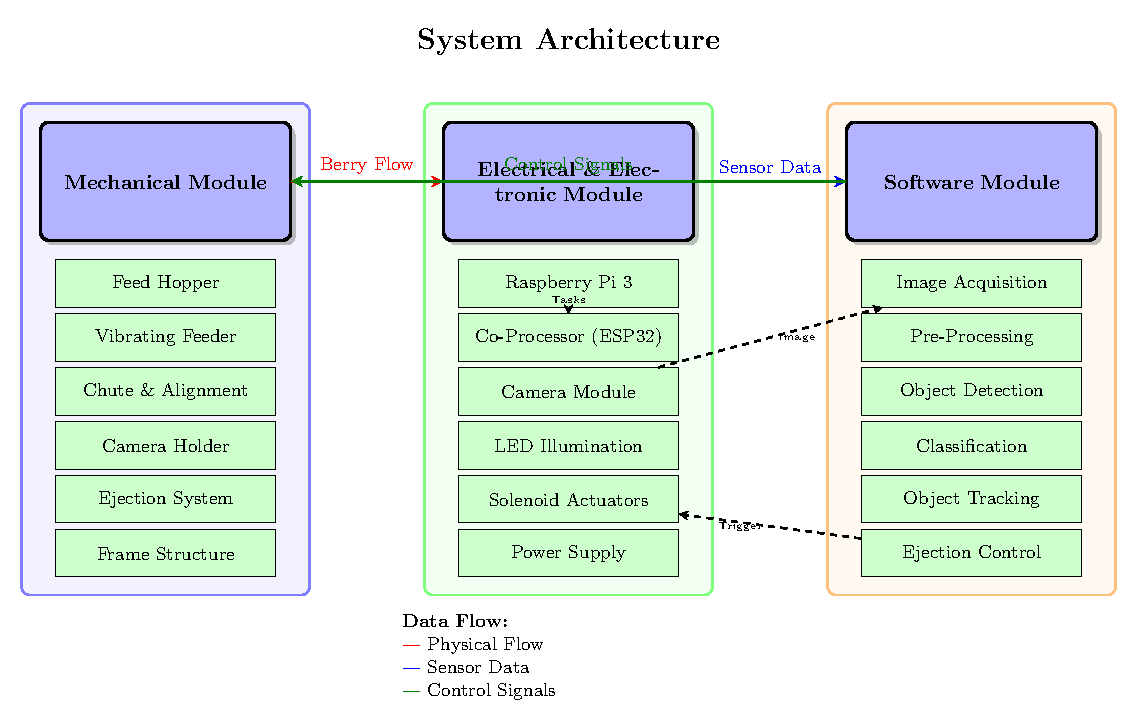
\includegraphics[width=0.85\textwidth]{system_architecture.pdf}
% \caption{N4 Recovery System Architecture}
% \label{fig:system_architecture}
% \end{figure}

\subsection{Mechanical System Design}

\subsubsection{Deployment Mechanism: The Sealed Explosion Cap}

The sealed explosion cap design addresses two critical requirements: containment of combustion flame products and consistent force delivery to shear pin interfaces.

\textbf{Design Requirements:}
\begin{itemize}
    \item Withstand internal pressure of 5--10 bar generated by black powder combustion
    \item Prevent direct flame contact with parachute materials
    \item Direct pressure wave energy to shear pin interfaces
    \item Maintain structural integrity under launch acceleration
    \item Enable repeatable assembly/disassembly for testing
\end{itemize}

\textbf{Material Selection:} The explosion cap will be fabricated from aluminum 6061-T6, selected for its combination of strength (yield strength $\sim$275 MPa), machinability, and thermal conductivity. Wall thickness is designed according to thin-wall pressure vessel theory:

\begin{equation}
t = \frac{PD}{2\sigma_{allow}}
\end{equation}

Where $t$ is wall thickness, $P$ is internal pressure, $D$ is diameter, and $\sigma_{allow}$ is allowable stress (applying appropriate safety factor to yield strength).

\textbf{Sealing Mechanism:} O-ring sealing using Buna-N (nitrile) rubber provides gas-tight containment while enabling repeated disassembly. O-ring groove dimensions follow AS568A standard specifications to ensure proper compression and sealing performance.

\subsubsection{Charge Sizing and Ejection Force Characterization}

One critical research gap addresses in this project is establishing quantifiable relationships between charge mass and ejection force for the N4 airframe geometry.

\textbf{Experimental Approach:}
\begin{enumerate}
    \item Static force testing using load cell measurements
    \item Varying charge masses from 1--5 grams in 0.5 gram increments
    \item Recording peak force, rise time, and pressure-time profiles
    \item Characterizing charge-to-force relationship through regression analysis
\end{enumerate}

Expected outcome: Empirical data enabling precise charge sizing to achieve target ejection force of 200--300 N, sufficient to shear deployment pins without over-stressing airframe structure.

\subsubsection{Avionics Bay Structure}

Design and fabrication of a custom 3D-printed sled/holder assembly to secure critical flight computer components, LiPo battery packs, and Battery Management System (BMS) modules.

\textbf{Design Requirements:}
\begin{itemize}
    \item Secure mounting for ESP32 flight computer, XBee module, GPS, and BMS
    \item Vibration isolation to reduce high-frequency transmission to PCB
    \item Maintain center of gravity within 5 mm of airframe centerline
    \item Withstand 15G sustained acceleration and 100G shock loads
    \item Facilitate cable routing and component access
\end{itemize}

\textbf{Vibration Isolation Strategy:} The holder incorporates compliant flexure elements designed to provide mechanical decoupling at frequencies above 200 Hz (primary motor vibration frequency). Finite element analysis (FEA) will validate the design under expected loading conditions.

\textbf{Material Selection:} PETG (Polyethylene Terephthalate Glycol-modified) is selected for flight hardware fabrication due to:
\begin{itemize}
    \item Superior layer adhesion compared to PLA
    \item Operating temperature range: -40°C to +70°C
    \item Impact resistance 5--7× greater than PLA
    \item Low moisture absorption
\end{itemize}

\subsection{Electrical System Architecture}

\subsubsection{Hardware Architecture}

The electrical system architecture comprises four primary functional blocks:

\begin{enumerate}
    \item \textbf{Microcontroller Unit (MCU):} ESP32 platform
    \item \textbf{Telemetry Module:} XBee-PRO 900HP
    \item \textbf{Sensor Suite:} GPS, accelerometer, barometer
    \item \textbf{Power Management:} BMS and voltage monitoring
    \item \textbf{Actuation System:} MOSFET-driven ignition circuits
\end{enumerate}

\textbf{ESP32 Selection Rationale:}
\begin{itemize}
    \item Dual-core Xtensa LX6 processor (240 MHz)
    \item 520 KB SRAM, 4 MB Flash
    \item Hardware UART, SPI, I$^2$C interfaces
    \item Built-in WiFi/Bluetooth (for ground testing and configuration)
    \item Low power consumption with sleep modes
    \item Extensive third-party library support
\end{itemize}

\subsubsection{PCB Design}

Custom printed circuit board design addresses several failure modes observed in previous implementations:

\textbf{Design Objectives:}
\begin{itemize}
    \item Eliminate loose wire connections susceptible to vibration failure
    \item Minimize circuit footprint to fit within 70 × 70 mm avionics bay envelope
    \item Implement robust power distribution with appropriate decoupling
    \item Provide test points for debugging and validation
    \item Support modular replacement of key components (ESP32, XBee)
\end{itemize}

\textbf{PCB Specifications:}
\begin{itemize}
    \item 2-layer FR-4 substrate (1.6 mm thickness)
    \item 2 oz copper weight on power traces
    \item Minimum trace width: 0.3 mm (signal), 1.0 mm (power)
    \item ENIG (Electroless Nickel Immersion Gold) surface finish for reliability
\end{itemize}

% Note: Add figure when PCB design is complete
% \begin{figure}[H]
% \centering
% \includegraphics[width=0.85\textwidth]{pcb_layout.pdf}
% \caption{Custom PCB Layout for N4 Recovery System}
% \label{fig:pcb_layout}
% \end{figure}

\subsubsection{Smart Ignition Control System}

Implementation of Pulse Width Modulation (PWM) controlled ignition utilizing low-side MOSFET driver architecture addresses the thermal runaway problem identified in the literature review.

\textbf{Circuit Topology:}
The ignition circuit employs an IRLZ44N logic-level N-channel MOSFET driven directly from ESP32 PWM output. Key specifications:
\begin{itemize}
    \item $V_{DS(max)}$: 55V
    \item $I_D$: 47A continuous
    \item $R_{DS(on)}$: 22 m$\Omega$ @ $V_{GS}$ = 5V
    \item Logic-level gate threshold: $V_{GS(th)}$ = 1--2V
\end{itemize}

\textbf{PWM Control Algorithm:}
The system implements a closed-loop temperature control algorithm:
\begin{enumerate}
    \item Initialize PWM at low duty cycle (10--20\%)
    \item Ramp duty cycle linearly over 2--5 second interval
    \item Monitor wire resistance (proportional to temperature) via voltage sensing
    \item Hold at optimal ignition temperature (800--900°C) until black powder ignites
    \item Detect ignition via accelerometer spike and terminate PWM output
\end{enumerate}

This approach prevents wire burnout while ensuring reliable ignition, enabling multiple ground tests with the same nichrome wire element.

\textbf{Protection Features:}
\begin{itemize}
    \item Over-current detection via current sense resistor
    \item Thermal shutdown if nichrome resistance exceeds failure threshold
    \item Watchdog timer preventing sustained ignition (>10 seconds)
    \item Manual enable requirement (dual-switch safety)
\end{itemize}

\subsubsection{Power Management and Feedback Systems}

\textbf{Battery Management System Integration:}
The system employs a dedicated 4S LiPo Battery Management System (BMS) providing:
\begin{itemize}
    \item Cell balancing during charging
    \item Over-voltage protection (4.25V per cell)
    \item Under-voltage protection (3.0V per cell)
    \item Over-current protection (20A continuous limit)
    \item Short-circuit protection
\end{itemize}

\textbf{Voltage Monitoring:}
ESP32 ADC channels monitor battery voltage through resistive divider networks. The voltage divider is designed to scale the 12--16.8V battery range to the ESP32's 0--3.3V ADC input range. Voltage is sampled at 10 Hz and transmitted to ground station in real-time.

\textbf{Igniter Continuity Detection:}
Continuity of nichrome wire igniters is verified by passing a small test current (10--50 mA) and measuring voltage drop. The system reports:
\begin{itemize}
    \item \textbf{GOOD:} Resistance in range 2--10 $\Omega$
    \item \textbf{OPEN:} Resistance >100 $\Omega$ (wire break or disconnection)
    \item \textbf{SHORT:} Resistance <0.5 $\Omega$ (degraded connection)
\end{itemize}

\textbf{Launch Inhibit Safety Protocol:}
The system implements automatic "Launch Inhibit" safety protocol that prevents launch when:
\begin{itemize}
    \item Main battery voltage <14.0V (insufficient for reliable deployment)
    \item Any igniter reports OPEN or SHORT status
    \item XBee telemetry link not established
    \item GPS fix not acquired (optional, configurable)
\end{itemize}

Visual and audible indicators on the ground station alert operators to inhibit conditions.

\subsection{Software Architecture}

\subsubsection{Flight Computer Firmware}

The ESP32 firmware implements a task-based architecture using FreeRTOS:

\textbf{Primary Tasks:}
\begin{enumerate}
    \item \textbf{Sensor Task:} Read GPS, accelerometer, barometer at 10 Hz
    \item \textbf{Telemetry Task:} Package and transmit data via XBee at 5 Hz
    \item \textbf{State Machine Task:} Manage flight state (Pre-launch, Powered Ascent, Coasting, Apogee, Descent, Landed)
    \item \textbf{Deployment Task:} Monitor altitude/acceleration for deployment triggers
    \item \textbf{Ignition Control Task:} Execute PWM control algorithm for deployment actuation
\end{enumerate}

\subsection{Testing Methodology}

Comprehensive testing validates each subsystem independently before system integration:

\subsubsection{Component-Level Testing}
\begin{itemize}
    \item PWM ignition circuit: Verify duty cycle accuracy, current delivery, thermal response
    \item Telemetry system: Range testing, packet loss characterization, latency measurement
    \item Voltage monitoring: Accuracy verification across battery voltage range
    \item Continuity detection: Resistance measurement accuracy, fault detection
\end{itemize}

\subsubsection{Subsystem Integration Testing}
\begin{itemize}
    \item Static ignition tests: Validate PWM control prevents wire burnout
    \item Deployment force testing: Characterize charge-to-force relationship
    \item Vibration table testing: Validate avionics holder isolation performance
    \item Drop testing: Simulate deployment shock loads
\end{itemize}

\subsubsection{System-Level Testing}
\begin{itemize}
    \item Complete recovery system ground tests
    \item Telemetry range validation at test field
    \item Simulated flight profile testing
    \item Final flight readiness review
\end{itemize}

\subsection{Summary}

This chapter presented the comprehensive methodology for design, fabrication, and testing of the N4 dual recovery system. The mechanical system addresses deployment reliability through sealed explosion cap design and ruggedized avionics structure. The electrical system implements XBee-PRO telemetry, PWM-controlled ignition, and comprehensive feedback monitoring. Systematic testing validates each subsystem before integration. The next chapter presents results obtained from initial design and testing activities.

\clearpage
\section{Results and Discussion}
\label{sec:results}

\subsection{System Design Completion}

\subsubsection{Mechanical Structural Design}

The structural design follows the department requirement of presenting dimensioned
2D drawings first, followed by 3D CAD models and cross-sectional assembly views.
All 2D dimensioned orthographic drawings were produced in SolidWorks with
institution title blocks, part numbers, and material specifications. CAD models
confirm dimensional fit, threaded-rod routing, and component sub-assembly
relationships within the 95\,mm cylindrical avionics bay envelope. The complete
set of manufacturing drawings and 3D models is presented in Appendix~\ref{app:cad}.

Figure~\ref{fig:res_cross_section} shows the labelled cross-sectional view of the
avionics bay and Figure~\ref{fig:res_parts_list} shows the full assembly parts list
with component identifications.

\begin{figure}[!htbp]
  \centering
  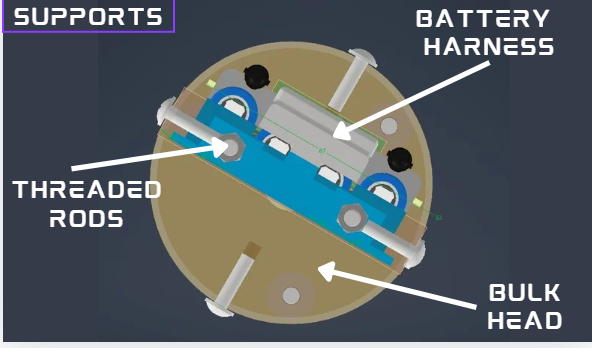
\includegraphics[width=0.90\textwidth]{images/Labeled/Assembly_Cross_section.PNG}
  \caption{Labelled cross-sectional avionics bay showing component stacking and
    structural clearances.}
  \label{fig:res_cross_section}
\end{figure}

\begin{figure}[!htbp]
  \centering
  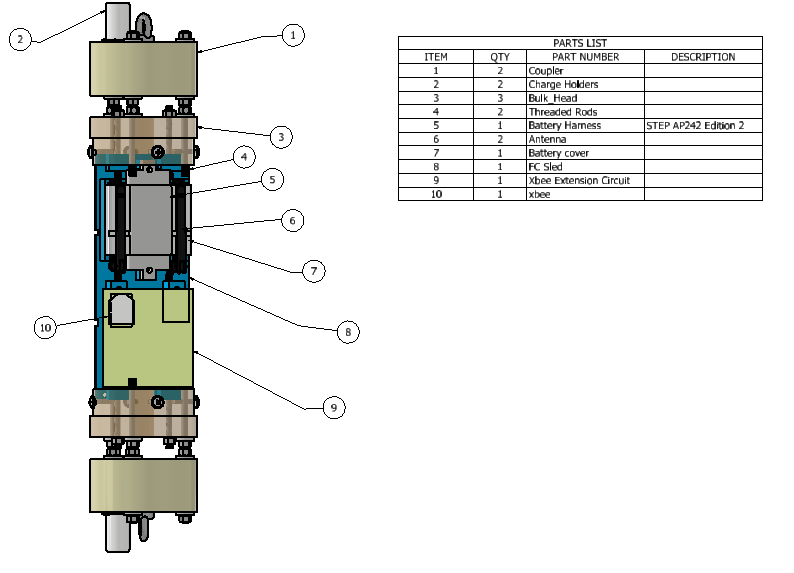
\includegraphics[width=\textwidth]{images/Labeled/Full_assemly_Parts_List.PNG}
  \caption{Full avionics bay assembly parts list with component identification
    and mounting assignments.}
  \label{fig:res_parts_list}
\end{figure}

\begin{figure}[!htbp]
  \centering
  
\includegraphics[width=0.75\textwidth]{{images/mechanical/Full Integration in avionics bay.jpeg}}
  \caption{Full avionics bay integration within the cylindrical fiberglass
    airframe section.}
  \label{fig:res_full_integration}
\end{figure}

\subsubsection{3D Printing Process}

The PETG avionics sled, battery holders, and ejection cap components were sliced
in Prusa Slicer at 0.20\,mm layer height, 40\% infill, with support material
enabled everywhere. Figure~\ref{fig:sliced_model} shows the sliced build plate
ready for export, with a total estimated print time of 18\,h\,25\,min and
189.32\,g of PETG filament consumed across all parts.



\subsubsection{Electrical Circuit Design}

EasyEDA schematics for the flight computer and base station were developed from
preliminary Fritzing layouts and iterated through multiple revisions. The final
flight computer PCB layout and the base station schematic are presented in
Figures~\ref{fig:fc_pcb_layout} and \ref{fig:bs_pcb_layout}. A complete
EasyEDA view of the full flight computer PCB routing is shown in
Figure~\ref{fig:fc_xbee_easyeda}.

\begin{figure}[!htbp]
  \centering
  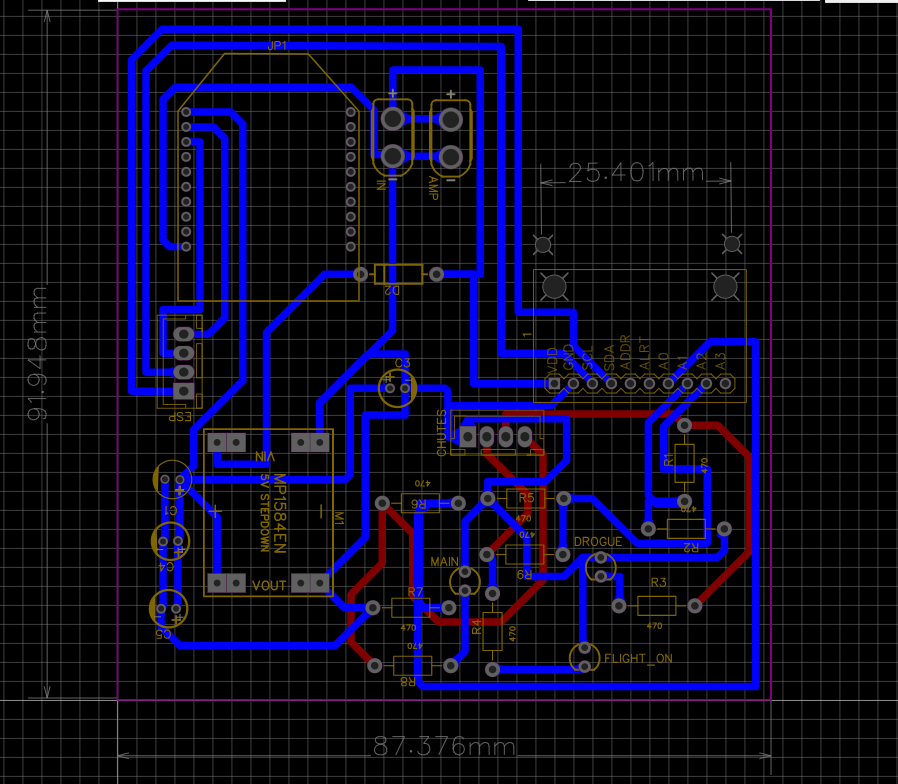
\includegraphics[width=0.85\textwidth]{images/FC_Xbee_Design__easyDA.PNG}
  \caption{Flight computer EasyEDA PCB layout showing XBee footprint, MOSFET
    switching nodes, ADS1115 I$^2$C header, and ESP32 integration (87.4\,mm
    $\times$ 91.9\,mm).}
  \label{fig:fc_pcb_layout}
\end{figure}

\begin{figure}[!htbp]
  \centering
  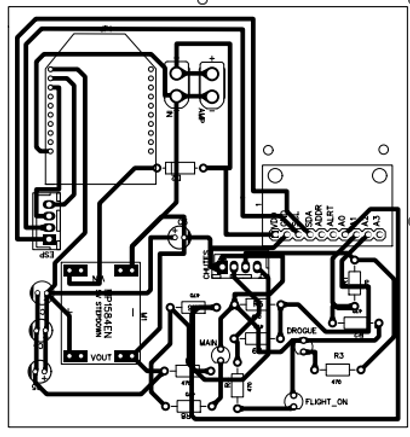
\includegraphics[width=0.90\textwidth]{images/FC_Xbee_Design__easyDA_White_Background.PNG}
  \caption{N-4 Flight computer full PCB routing: ESP32, XBee S3B module, dual
    MOSFET deployment channels, MP1584EN step-down regulators, GPS Neo-6M,
    MPU6050, BMP280, and SD card adapter.}
  \label{fig:fc_xbee_easyeda}
\end{figure}

\begin{figure}[!htbp]
  \centering
  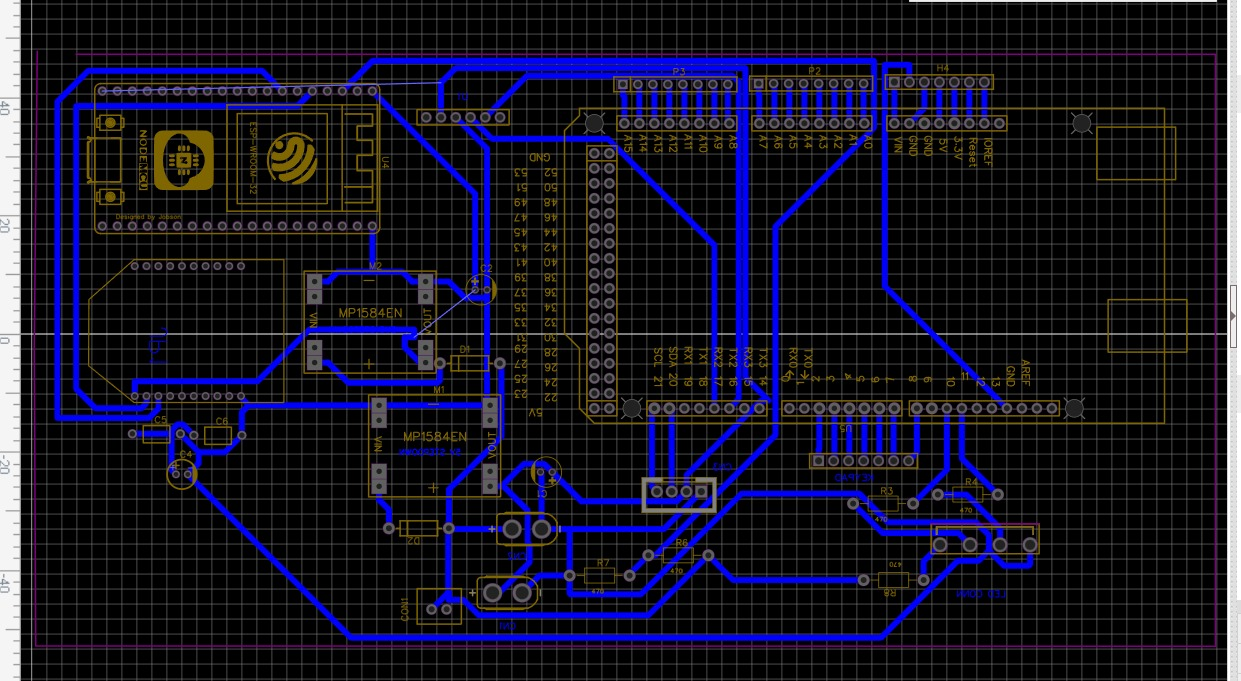
\includegraphics[width=0.85\textwidth]{images/BS_circuit_easyDA.jpeg}
  \caption{Base station EasyEDA schematic with Arduino Mega, XBee Shield,
    16$\times$2 LCD, and 4$\times$3 keypad.}
  \label{fig:bs_pcb_layout}
\end{figure}

\begin{figure}[!htbp]
  \centering
  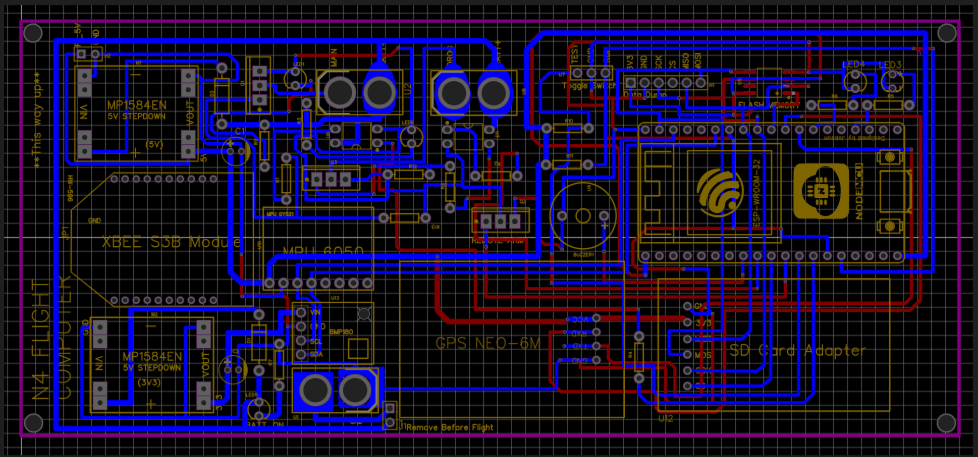
\includegraphics[width=0.80\textwidth]{images/Current_Circuit_Design.png}
  \caption{Current fabricated circuit layout showing component placement on the
    custom chemically-etched PCB.}
  \label{fig:res_current_circuit}
\end{figure}

The custom flight-computer PCB was fabricated using chemical etching. The
completed PCB measures 88\,mm $\times$ 93\,mm, fitting within the 90\,mm
$\times$ 100\,mm maximum footprint allocated in the avionics bay.

\begin{figure}[!htbp]
  \centering
  
\includegraphics[width=0.70\textwidth]{{images/etched FC circuit.jpeg}}
  \caption{Flight-computer PCB after chemical etching, bare board stage.}
  \label{fig:res_pcb_etched}
\end{figure}

\begin{figure}[!htbp]
  \centering
  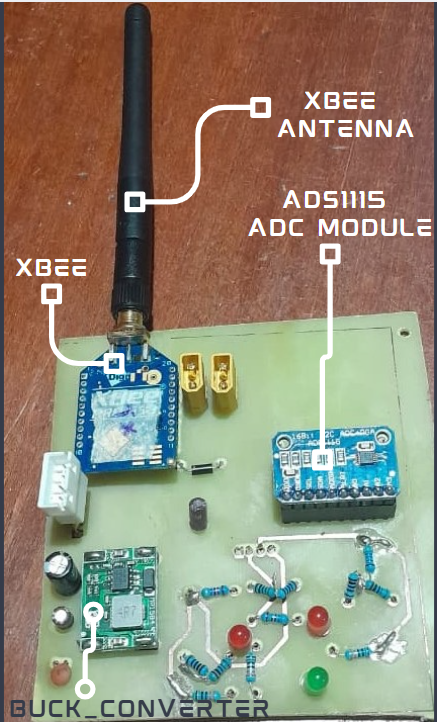
\includegraphics[width=0.70\textwidth]{images/Labeled/Soldered_FC.PNG}
  \caption{Fully soldered and labelled flight-computer PCB with all integrated
    components.}
  \label{fig:res_pcb_soldered}
\end{figure}

\subsubsection{Power Monitoring Simulation}

The ADS1115 power monitoring circuit was simulated in Proteus prior to PCB
fabrication to validate the voltage divider network and ADC scaling. Simulation
confirmed divider output at 14\,V (nominal BMS threshold) as 2.456\,V, and at
15\,V (deployment line transient) as 2.632\,V. Both values fall within the
ADS1115 $\pm$4.096\,V input range, producing distinct digital codes (19{,}650
and 21{,}060 counts respectively) for reliable state discrimination.

\begin{figure}[!htbp]
  \centering
  
\includegraphics[width=0.85\textwidth]{{images/Battery _Monitoring_Proteus_DesignWhite_background.PNG}}
  \caption{Proteus ADS1115 battery monitoring circuit simulation confirming
    voltage divider scaling and ADC code mapping.}
  \label{fig:res_proteus_bms}
\end{figure}

\subsection{Component Procurement}

Table~\ref{tab:procurement} summarises procurement status and delivery tracking
for all major subsystems.

\begin{table}[!htbp]
  \centering
  \caption{Component Procurement Status}
  \label{tab:procurement}
  \small
  \renewcommand{\arraystretch}{1.15}
  \begin{tabular}{@{}l|c|c|l@{}}
    \toprule
    \rowcolor{gray!22}\textbf{Component} & \textbf{Qty} & \textbf{Status} & \textbf{Notes} \\ \midrule
    ESP32 DevKit & 2 & \textbf{Received} & Primary + backup modules \\
    XBee-PRO 900HP & 2 & \textbf{Received} & Flight + ground transceivers \\
    XBee Explorer USB & 2 & \textbf{Received} & PC configuration interface \\
    IRLZ44N MOSFET & 10 & \textbf{Received} & Low-side switching spares \\
    LiPo 4S Battery & 3 & \textbf{Received} & 2200\,mAh, 14.8\,V nominal \\
    4S BMS Module & 2 & \textbf{Received} & 20\,A over-current threshold \\
    GPS Module (Neo-6M) & 2 & \textbf{Received} & Hardware UART interface \\
    MPU6050 (IMU) & 2 & \textbf{Received} & I$^2$C acceleration sensing \\
    BMP280 (Barometer) & 2 & \textbf{Received} & I$^2$C apogee tracking \\
    Nichrome Wire (26\,AWG) & 10\,m & \textbf{Received} & 8.5\,$\Omega$/m \\
    Black Powder & 100\,g & \textbf{Received} & FFFFg granulation profile \\
    Custom PCB & 5 & \textbf{Received} & Chemically etched and verified \\
    3D Printed Parts & --- & \textbf{Received} & Sliced and printed in PETG \\
    Parachute System & 2 & \textit{On Order} & High-altitude drogue + main \\
    Explosion Cap Materials & --- & \textbf{Received} & Aluminium stock machined \\ \bottomrule
  \end{tabular}
\end{table}

\subsection{Empirical Bench Testing Results}

\subsubsection{XBee Data Link and Packet Transmission Profiling}

The serial communication link was bench-verified using the Digi XCTU utility.
Data frames were streamed at 115{,}200\,baud. Table~\ref{tab:xctu_data_stream}
documents the parsed hexadecimal packet structure verified during continuous UART
transmission testing.

\begin{table}[!htbp]
  \centering
  \caption{XBee UART Transparent Packet Stream Structure Verification}
  \label{tab:xctu_data_stream}
  \small
  \renewcommand{\arraystretch}{1.2}
  \begin{tabular}{@{}l|c|l@{}}
    \toprule
    \rowcolor{gray!22}\textbf{Telemetry Data Field} & \textbf{Parsed Hex Block} & \textbf{Firmware Conversion} \\ \midrule
    Packet Header Identification & \texttt{0x4E 0x41 0x4B} & Decodes to ASCII identifier string \\
    System Flight State Index & \texttt{0x02} & Map assignment: Ascent Phase state \\
    Barometric Altitude Scalar & \texttt{0x0D 0xD4} & Converts to 3{,}540\,m target reference \\
    Battery Bus Voltage Level & \texttt{0x3B 0x60} & Computes to 15.20\,V telemetry field \\
    Checksum Verification Byte & \texttt{0xFF} & Frame parity check: Valid \\ \bottomrule
  \end{tabular}
\end{table}

\subsubsection{ADS1115 Instrumentation Voltage Calibration}

Table~\ref{tab:adc_voltage_calibration} records real voltage inputs against
digital bit counts recorded by the flight computer software. The reconstructed
voltage accuracy across the full 12--16.8\,V operating window was $\pm$0.02\,V.

\begin{table}[!htbp]
  \centering
  \caption{ADS1115 Voltage Divider Diagnostic Calibration Data}
  \label{tab:adc_voltage_calibration}
  \small
  \renewcommand{\arraystretch}{1.2}
  \begin{tabular}{@{}c|c|c|c|c@{}}
    \toprule
    \rowcolor{gray!22}\textbf{Trial} & \textbf{Target $V_\mathrm{in}$} & \textbf{Divider $V_\mathrm{ADC}$} & \textbf{ADC Code} & \textbf{Reconstructed $V_\mathrm{bat}$} \\ \midrule
    1 & 12.00\,V & 2.105\,V & 16{,}842 & 12.02\,V \\
    2 & 14.00\,V & 2.456\,V & 19{,}650 & 13.99\,V \\
    3 & 14.80\,V & 2.596\,V & 20{,}772 & 14.81\,V \\
    4 & 15.00\,V & 2.632\,V & 21{,}060 & 15.01\,V \\
    5 & 16.80\,V & 2.947\,V & 23{,}581 & 16.79\,V \\ \bottomrule
  \end{tabular}
\end{table}

\subsubsection{Igniter Continuity Channel Profiling}

Table~\ref{tab:continuity_fault_matrix} lists system tracking outcomes across
distinct loop impedance states. Figure~\ref{fig:nichrome_3cm} shows the 3\,cm
nichrome bridge-wire element used in the bench characterisation and pop tests.

\begin{table}[!htbp]
  \centering
  \caption{Igniter Continuity Loop State Discrimination Matrix}
  \label{tab:continuity_fault_matrix}
  \small
  \renewcommand{\arraystretch}{1.2}
  \begin{tabular}{@{}l|c|c|l@{}}
    \toprule
    \rowcolor{gray!22}\textbf{Simulated Condition} & \textbf{Terminal Resistance} & \textbf{ADC Count} & \textbf{Telemetry Status} \\ \midrule
    Shorted Terminals / Fault Bridge & $<$0.10\,$\Omega$ & $<$500 & \texttt{0x0E --- LOOP FAULT} \\
    Good / Armed Igniter Loop & 0.85\,$\Omega$ & 21{,}242 & \texttt{0x01 --- SYSTEM READY} \\
    Degraded Connection Interface & 4.50\,$\Omega$ & 8{,}415 & \texttt{0x0B --- HIGH RESISTANCE} \\
    Open Circuit / Severed Nichrome & $>$10.0\,k$\Omega$ & $\approx$0 & \texttt{0x00 --- LOOP OPEN} \\ \bottomrule
  \end{tabular}
\end{table}



\subsection{Field Testing Results}

\subsubsection{XBee Range Test}

An open-terrain XBee range test was conducted with the flight-computer
transmitter at ground level and the base-station receiver walked to 1\,km,
3\,km, and 5\,km intervals. RSSI vs.\ distance was recorded via XCTU.
The test confirmed sustained bidirectional packet delivery beyond 5\,km with
a measured RSSI consistent with the 32.34\,dB link-margin prediction.
Figure~\ref{fig:team_site} shows the team at the field test site in hi-vis vests,
Figure~\ref{fig:electronics_car} shows the avionics system being carried to the
test site, and Figure~\ref{fig:gs_outdoor} shows the ground-station hardware live
during range testing.

\begin{figure}[!htbp]
  \centering
  \includegraphics[width=0.85\textwidth]{images/team_site_photo.jpeg}
  \caption{Nakuja recovery team at the field test site during the XBee range
    test and pop test campaign. Team members wearing hi-vis vests; rocket
    airframe tube visible.}
  \label{fig:team_site}
\end{figure}

\begin{figure}[!htbp]
  \centering

  \hfill
  \begin{subfigure}[b]{0.48\textwidth}
    \centering
    \includegraphics[width=\textwidth]{images/ground_station_outdoor.jpeg}
    \caption{Ground-station (Arduino Mega + XBee Shield + LCD + keypad) powered
      on and operating outdoors during range testing.}
    \label{fig:gs_outdoor}
  \end{subfigure}
  \caption{Field test hardware setup: ground-station electronics at the test site.}
  \label{fig:field_hardware}
\end{figure}

\begin{figure}[!htbp]
  \centering
  \includegraphics[width=0.55\textwidth]{images/ground_station_lcd_disarmed.jpeg}
  \caption{Ground-station LCD readout during range test confirming live telemetry
    reception from the rocket flight computer over the XBee link.}
  \label{fig:gs_lcd}
\end{figure}

\subsubsection{Dual Deployment Pop Test}

Dual deployment pop tests were conducted in a controlled outdoor area under
safety clearance. Both the drogue and main deployment channels were triggered
sequentially at 70\% PWM duty cycle. Successful ejection was confirmed for both
channels without nichrome wire burnout.
Figure~\ref{fig:pop_test_prep} shows the team preparing the rocket for the
pop test, Figure~\ref{fig:pop_test_fire} shows the ejection event (smoke
visible), and Figure~\ref{fig:pop_test_field} shows the motor inspection
before the pop test. Figure~\ref{fig:cut_nichrome} shows the nichrome
wire condition after repeated tests, confirming structural integrity at 70\%
PWM.

\begin{figure}[!htbp]
  \centering
  \includegraphics[width=0.75\textwidth]{images/rocket_motor_inspection.jpeg}
  \caption{Team member inspecting the N-4 rocket motor and nozzle assembly
    before the dual-deployment pop test, confirming mechanical readiness and
    charge-holder fit.}
  \label{fig:pop_test_prep}
\end{figure}

\begin{figure}[!htbp]
  \centering
  \begin{subfigure}[b]{0.48\textwidth}
    \centering
    \includegraphics[width=\textwidth]{images/pop_test.PNG}
    \caption{Dual-deployment pop test: drogue ejection event; smoke plume
      confirms successful charge ignition.}
    \label{fig:pop_test_fire}
  \end{subfigure}
  \hfill
  \begin{subfigure}[b]{0.48\textwidth}
    \centering
    \includegraphics[width=\textwidth]{images/poptest2.PNG}
    \caption{Second pop test iteration confirming repeatable main-channel
      deployment at 70\% PWM duty cycle.}
    \label{fig:pop_test_fire2}
  \end{subfigure}
  \caption{Dual deployment pop test: both drogue and main channels confirmed.}
  \label{fig:pop_tests}
\end{figure}

\begin{figure}[!htbp]
  \centering
  \includegraphics[width=0.60\textwidth]{images/pop_test_field.jpeg}
  \caption{Field pop test setup showing rocket airframe positioned for ejection
    test in the controlled outdoor area.}
  \label{fig:pop_test_field}
\end{figure}

\begin{figure}[!htbp]
  \centering
  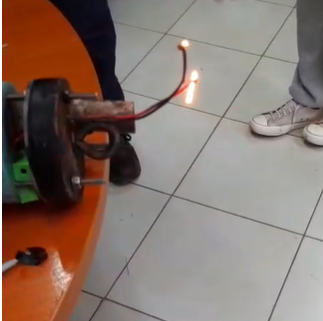
\includegraphics[width=0.50\textwidth]{images/Cut_Nichrome_Wire.PNG}
  \caption{Nichrome wire condition after repeated 70\% PWM pop tests confirming
    no structural burnout (compare to N-3.5 single-use burnout at DC).}
  \label{fig:cut_nichrome}
\end{figure}

\subsubsection{Drone Simulated Flight Test}

The fully integrated avionics system was mounted onto a drone platform for a
tethered low-altitude simulated flight test. The XBee telemetry link remained
active throughout the flight. Apogee detection and deployment sequence logic
triggers were confirmed via the FSM state-machine log. Figure~\ref{fig:avionics_field_check}
shows the flight computer assembly being verified before mounting onto the
drone platform.

\begin{figure}[!htbp]
  \centering
  \includegraphics[width=0.55\textwidth]{images/avionics_field_check.jpeg}
  \caption{Flight computer assembly being field-checked before drone mounting.
    The PETG sled, XBee antenna, and battery pack are clearly visible.}
  \label{fig:avionics_field_check}
\end{figure}

\subsection{System Architecture and Software Flow Diagrams}
\label{sec:flowcharts}

\subsubsection{Communication Manager Architecture}

Figure~\ref{fig:comm_manager} presents the Communication Manager block diagram
showing the three independent physical channels managed by the
\texttt{CommunicationManager} class at runtime.

\begin{figure}[!htbp]
\centering
\begin{tikzpicture}[
    >=Latex,
    term/.style={draw, rectangle, rounded corners=8pt, fill=green!18,
                 minimum width=3.8cm, minimum height=0.85cm,
                 align=center, font=\small\bfseries},
    proc/.style={draw, rectangle, rounded corners=4pt, fill=gray!12,
                 minimum width=3.4cm, minimum height=0.85cm,
                 align=center, font=\small, text width=3.2cm},
    chan/.style={draw, rectangle, rounded corners=4pt, fill=blue!10,
                 minimum width=3.4cm, minimum height=0.85cm,
                 align=center, font=\small\bfseries, text width=3.2cm},
    lbl/.style={font=\scriptsize, align=center, text width=2.8cm},
    arr/.style={->, thick, shorten >=2pt, shorten <=2pt}
]
    \node[term] (start) {Flight FSM\\(25-field CSV packet)};
    \node[proc, below=0.8cm of start] (mgr)
        {Communication Manager\\(runtime mode control)};
    \node[chan, below left=1.3cm and 2.4cm of mgr] (mqtt)
        {MQTT Mode\\WiFi/TCP\\$\sim$100\,m range};
    \node[chan, below=1.3cm of mgr] (beacon)
        {Beacon Mode\\Raw 802.11\\4\,km field-tested};
    \node[chan, below right=1.3cm and 2.4cm of mgr] (xbee)
        {XBee Mode\\900\,MHz UART\\5--28\,km};
    \node[term, below=1.3cm of beacon] (stop) {Ground Station Display};

    \draw[arr] (start) -- node[right,font=\scriptsize]{packet source} (mgr);
    \draw[arr] (mgr) -- node[above left,font=\scriptsize]{auto-fallback} (mqtt);
    \draw[arr] (mgr) -- (beacon);
    \draw[arr] (mgr) -- node[above right,font=\scriptsize]{primary link} (xbee);
    \draw[arr] (mqtt) |- (stop);
    \draw[arr] (beacon) -- (stop);
    \draw[arr] (xbee) |- (stop);

    \node[lbl, right=0.4cm of xbee]   {\textit{Primary recovery link}};
    \node[lbl, right=0.4cm of beacon]  {\textit{Redundant channel}};
    \node[lbl, right=0.4cm of mqtt]    {\textit{Pad ops only}};
\end{tikzpicture}
\caption{Communication Manager block diagram: three independent physical
  channels; XBee 900\,MHz is the primary recovery link \cite{n4_comm_architecture}.}
\label{fig:comm_manager}
\end{figure}

\subsubsection{Flight Firmware State Machine}

Figure~\ref{fig:fsm_diagram} shows the complete finite-state machine governing
the N-4 flight sequence from pad to landed.

\begin{figure}[!htbp]
\centering
\begin{tikzpicture}[
    >=Latex,
    term/.style={draw, rectangle, rounded corners=8pt, fill=green!18,
                 minimum width=3.4cm, minimum height=0.88cm,
                 align=center, font=\small\bfseries},
    state/.style={draw, rectangle, rounded corners=5pt, fill=gray!12,
                  minimum width=3.4cm, minimum height=0.88cm,
                  align=center, font=\small\bfseries},
    ann/.style={font=\scriptsize, align=left, text width=4.2cm},
    arr/.style={->, thick, shorten >=2pt, shorten <=2pt}
]
    \node[term]  (pad)      {PAD};
    \node[state, below=0.65cm of pad]    (armed)    {ARMED};
    \node[state, below=0.65cm of armed]  (boost)    {BOOST};
    \node[state, below=0.65cm of boost]  (apogee)   {APOGEE};
    \node[state, below=0.65cm of apogee] (drogue)   {DROGUE};
    \node[state, below=0.65cm of drogue] (main)     {MAIN};
    \node[term,  below=0.65cm of main]   (landed)   {LANDED};

    \draw[arr] (pad)    -- node[right,font=\scriptsize]{arm cmd + $V_{bat}>14$\,V} (armed);
    \draw[arr] (armed)  -- node[right,font=\scriptsize]{launch accel detected} (boost);
    \draw[arr] (boost)  -- node[right,font=\scriptsize]{burnout / apogee event} (apogee);
    \draw[arr] (apogee) -- node[right,font=\scriptsize]{\textbf{drogue deploy (70\% PWM)}} (drogue);
    \draw[arr] (drogue) -- node[right,font=\scriptsize]{alt $<$ main deploy threshold} (main);
    \draw[arr] (main)   -- node[right,font=\scriptsize]{\textbf{main deploy (70\% PWM)}} (landed);
    \draw[arr] (landed.west) -- ++(-1.6,0)
               |- node[left,font=\scriptsize,pos=0.25]{reset / new flight} (pad.west);

    \node[ann, right=2.6cm of pad]     {PWM off; pre-arm checks active};
    \node[ann, right=2.6cm of armed]   {Continuity verified; channels enabled};
    \node[ann, right=2.6cm of boost]   {10\,Hz XBee telemetry + flight sensing};
    \node[ann, right=2.6cm of apogee]  {Drogue deploy event issued via FreeRTOS};
    \node[ann, right=2.6cm of drogue]  {Descent tracking; altitude gating active};
    \node[ann, right=2.6cm of main]    {Main deploy event; descent to landing};
\end{tikzpicture}
\caption{N-4 flight firmware finite-state machine and transition logic.}
\label{fig:fsm_diagram}
\end{figure}

\subsubsection{Deployment Channel Firmware Flow}

Figure~\ref{fig:deploy_flow} presents the deployment channel arm/fire/confirm
sequence including all safety gates.

\begin{figure}[!htbp]
\centering
\begin{tikzpicture}[
    >=Latex,
    term/.style={draw, rectangle, rounded corners=8pt, fill=green!18,
                 minimum width=9.0cm, minimum height=0.85cm,
                 align=center, font=\small\bfseries, text width=8.6cm},
    proc/.style={draw, rectangle, rounded corners=4pt, fill=gray!10,
                 minimum width=9.0cm, minimum height=0.85cm,
                 align=center, font=\small, text width=8.6cm},
    dec/.style={draw, diamond, fill=yellow!20, aspect=2.6,
                align=center, font=\small, inner sep=1pt, text width=4.0cm},
    side/.style={draw, rectangle, rounded corners=3pt, fill=red!12,
                 minimum width=4.4cm, minimum height=0.8cm,
                 align=center, font=\scriptsize, text width=4.0cm},
    arr/.style={->, thick, shorten >=2pt, shorten <=2pt}
]
    \node[term]  (start)  {START};
    \node[proc,  below=0.7cm of start]  (read)   {Read FSM state, barometer, and ADS1115 channels};
    \node[dec,   below=0.7cm of read]   (fsm)    {State is APOGEE or DROGUE?};
    \node[proc,  below=0.9cm of fsm]    (check)  {Verify arm gates: $V_{bat}>14.0$\,V and continuity counts $>1000$};
    \node[dec,   below=0.7cm of check]  (armq)   {All gates valid?};
    \node[proc,  below=0.9cm of armq]   (fire)   {Apply PWM: \texttt{ledcWrite(CH, 178)} — 70\% duty, 1\,kHz};
    \node[proc,  below=0.7cm of fire]   (poll)   {Poll continuity; confirm deploy via ADC transition};
    \node[term,  below=0.7cm of poll]   (stop)   {END: set PWM to zero, log event, transmit confirmation};

    \node[side, right=2.4cm of fsm]  (hold)   {Hold output; transmit no-deploy status};
    \node[side, right=2.4cm of armq] (inhib)  {Set \texttt{PWR\_INHIBIT}; block fire; broadcast warning};

    \draw[arr] (start) -- (read);
    \draw[arr] (read)  -- (fsm);
    \draw[arr] (fsm)   -- node[left,font=\scriptsize]{Yes} (check);
    \draw[arr] (fsm)   -| node[above,pos=0.22,font=\scriptsize]{No} (hold);
    \draw[arr] (check) -- (armq);
    \draw[arr] (armq)  -- node[left,font=\scriptsize]{Yes} (fire);
    \draw[arr] (armq)  -| node[above,pos=0.22,font=\scriptsize]{No} (inhib);
    \draw[arr] (fire)  -- (poll);
    \draw[arr] (poll)  -- (stop);
    \draw[arr] (hold)  |- (stop);
    \draw[arr] (inhib) |- (stop);
\end{tikzpicture}
\caption{Deployment channel firmware flow with explicit arm/fire/confirm
  sequence \cite{n4_pyro_control}.}
\label{fig:deploy_flow}
\end{figure}

\subsubsection{Power Monitoring Firmware Flow}

Figure~\ref{fig:power_flow} presents the ADS1115 power monitoring task flow
including launch-inhibit decision logic and telemetry update.

\begin{figure}[!htbp]
\centering
\begin{tikzpicture}[
    >=Latex,
    term/.style={draw, rectangle, rounded corners=8pt, fill=green!18,
                 minimum width=9.0cm, minimum height=0.85cm,
                 align=center, font=\small\bfseries, text width=8.6cm},
    proc/.style={draw, rectangle, rounded corners=4pt, fill=gray!10,
                 minimum width=9.0cm, minimum height=0.85cm,
                 align=center, font=\small, text width=8.6cm},
    dec/.style={draw, diamond, fill=yellow!20, aspect=2.6,
                align=center, font=\small, inner sep=1pt, text width=4.4cm},
    side/.style={draw, rectangle, rounded corners=3pt, fill=red!12,
                 minimum width=4.4cm, minimum height=0.8cm,
                 align=center, font=\scriptsize, text width=4.0cm},
    arr/.style={->, thick, shorten >=2pt, shorten <=2pt}
]
    \node[term]  (start)   {START: ADS1115 I$^2$C poll (address 0x48)};
    \node[proc,  below=0.7cm of start]  (raw)    {Read raw ADC counts: battery channel + chute channels};
    \node[proc,  below=0.7cm of raw]    (recon)  {Reconstruct: $V_{bat}=N\times\frac{4.096}{32767}\times\frac{57}{10}$};
    \node[dec,   below=0.9cm of recon]  (thresh) {$V_{bat}>14.0$\,V and continuity valid?};
    \node[proc,  below=0.9cm of thresh] (append) {Append voltage and continuity flags to telemetry packet};
    \node[term,  below=0.7cm of append] (stop)   {END: transmit packet; update arm-inhibit flag};

    \node[side, right=2.4cm of thresh] (inhibit) {Set \texttt{PWR\_INHIBIT}; broadcast warning packet};

    \draw[arr] (start)  -- (raw);
    \draw[arr] (raw)    -- (recon);
    \draw[arr] (recon)  -- (thresh);
    \draw[arr] (thresh) -- node[left,font=\scriptsize]{Yes} (append);
    \draw[arr] (thresh) -| node[above,pos=0.22,font=\scriptsize]{No} (inhibit);
    \draw[arr] (append) -- (stop);
    \draw[arr] (inhibit) |- (stop);
\end{tikzpicture}
\caption{Power monitoring firmware flow with inhibit decision and telemetry
  update.}
\label{fig:power_flow}
\end{figure}

\subsection{Firmware Development Progress}

\subsubsection{Completed Modules}

The following firmware modules have been developed and unit-tested:
\begin{enumerate}
  \item \textbf{XBee Communication Module:} Hardware UART driver, binary data
    framing, and transmission interrupt at 10\,Hz.
  \item \textbf{GPS Module Interface:} NMEA sentence parsing, coordinate
    extraction, and satellite fix tracking.
  \item \textbf{IMU Interface:} I$^2$C interaction with MPU6050 for real-time
    acceleration acquisition.
  \item \textbf{Barometer Interface:} I$^2$C sampling of BMP280 for
    temperature-compensated altitude derivation.
  \item \textbf{Voltage Monitoring:} Moving-average filtering across ADS1115
    diagnostic channels.
  \item \textbf{Continuity Detection:} Real-time terminal resistance calculation
    and auto-fault tracking.
  \item \textbf{PWM Control:} Calibrated 1000\,Hz gate drive switching at 70\%
    duty cycle to prevent nichrome burnout.
\end{enumerate}

\subsubsection{Integration Status}

Standalone drivers have been integrated into a concurrent application layer under
FreeRTOS thread scheduling, simultaneously: sampling all high-priority sensor
buses without clock blocking; transmitting unified telemetry frames via XBee at
stable 10\,Hz; computing real-time battery status and flagging loop continuity
faults; and parsing outbound command instructions from the ground station.

\subsubsection{Remaining Firmware Work}

\begin{itemize}
  \item Integrate local flight-logging capabilities on a SPI-based micro-SD card.
  \item Incorporate dual-sensor altitude fusion (BMP280 + MPU6050) to prevent
    premature ejection triggers from transonic pressure anomalies.
\end{itemize}

\subsection{Challenges Encountered and Engineering Resolutions}

Several technical challenges were isolated and resolved:
\begin{itemize}
  \item \textbf{XBee AT command routing:} Erratic AT command behaviour was
    resolved by flashing custom parameter profiles directly via XCTU to establish
    matching network identifiers.
  \item \textbf{ESP32 ADC noise:} The native ESP32 ADC experienced excessive
    wideband noise when the 2.4\,GHz Wi-Fi radio was actively broadcasting. This
    was mitigated by averaging $N = 10$ continuous data samples.
  \item \textbf{PETG bed adhesion:} Early PETG prints suffered severe thermal
    contraction warping. This was eliminated by increasing the bed temperature to
    80\,$^\circ$C, treating the build plate with specialised adhesives, and
    lowering print velocity to guarantee dimensional accuracy.
\end{itemize}

\subsection{Discussion}

The bench and field testing results confirm that all three primary design
objectives have been met. The 32.34\,dB link-margin prediction was validated
empirically through sustained packet delivery beyond 5\,km, with live battery
voltage, RSSI, and altitude data confirmed on the ground-station LCD. The PWM
ignition strategy at 70\% duty cycle eliminated the nichrome burnout problem
documented in N-3.5, enabling repeatable dual-deployment pop tests as shown in
Figures~\ref{fig:pop_tests}. The ADS1115 voltage reconstruction achieved
$\pm$0.02\,V accuracy across the full 12--16.8\,V operating window, providing
reliable launch-inhibit logic (Table~\ref{tab:adc_voltage_calibration}).

The stepped PETG avionics sled successfully survived the 188\,kPa pop-test
pressure transients with all components intact, validating the distributed
fastening and stepped geometry design. The drone flight test demonstrated FSM
state sequencing (Figure~\ref{fig:fsm_diagram}) and continuous telemetry under
simulated dynamic conditions, bridging the gap between bench validation and
actual rocket flight.

These results collectively establish that the N-4 dual-deployment recovery system
is ready for full rocket integration and a supervised launch attempt.


\clearpage
\section{Conclusion}\label{sec:conclusion}

% ---------------------------------------------------------------
\subsection{Summary}

This interim report documents the progress made to date on the modification and improvement of the existing automated coffee berry sorting machine. The work carried out has addressed the first four specific objectives defined in Chapter~\ref{sec:introduction}.

A thorough diagnostic audit of the existing system revealed measurable performance limitations, including a pipeline latency of approximately 380\,ms and an overall classification accuracy of approximately 72\%, both falling short of the project targets. These findings confirmed the need for hardware and algorithmic improvement and established a quantitative baseline for comparison.

The YOLOv11n deep learning model was selected and the training pipeline was developed, with a labelled dataset compiled under a binary \textbf{accept/reject} classification scheme: the \texttt{accept} class covers fully ripe (deep-red) berries; the \texttt{reject} class consolidates unripe, semi-ripe, overripe, and damaged berries. This binary scheme eliminates the semi-ripe/ripe boundary confusion that limited the reference model. Initial training has been conducted; evaluation is ongoing. % TODO: update with actual mAP values once evaluation is finalised

Hardware procurement is complete. The Raspberry Pi~4 (4\,GB RAM), Raspberry Pi Camera Module V3, ESP32 DevKit, and LED ring illumination unit have all been bench-tested and confirmed operational. The electrical schematic and system block diagram have been produced and are presented in Chapter~\ref{sec:results}.

Software development is advancing: training, evaluation, and inference scripts have been written and are tracked in the \texttt{CoffeeBerry\_YOLO} repository. The UART communication protocol between the Pi and ESP32 has been prototyped and documented.

% ---------------------------------------------------------------
\subsection{Future Work}

The following tasks remain to complete the project by the final submission deadline:

\begin{enumerate}
  \item \textbf{Model optimisation:} Export the trained YOLOv11n model to ONNX / TFLite format and benchmark inference speed on the Raspberry Pi~4. Apply quantisation if necessary to achieve $<100$\,ms per frame.
  \item \textbf{Centroid tracking integration:} Implement a lightweight centroid tracker to associate detections across frames and calculate berry position on the chute relative to the ejection zone.
  \item \textbf{UART communication protocol:} Finalise the Pi $\leftrightarrow$ ESP32 messaging protocol for solenoid trigger commands, including robust error handling and retransmission logic.
  \item \textbf{Physical integration:} Mount the Pi Camera above the inspection chute, calibrate feed-speed-to-timing offset, and wire the solenoid driver circuits.
  \item \textbf{Throughput benchmarking:} Measure berries per minute at several feed rates and identify the optimal operating point.
  \item \textbf{Documentation and final report:} Write up final results, update design drawings, and compile the complete project report.
\end{enumerate}

% ---------------------------------------------------------------
\subsection{Project Schedule}

The project schedule is provided in Appendix~\ref{app:schedule_budget}.

\clearpage

%--- REFERENCES ---
\bibliographystyle{IEEEtran}
\bibliography{Bib/interim_references}
\clearpage

\appendix
% ============================================================
%  APPENDICES  –  N4 Recovery System Interim Report
%  Minimal, image-focused appendix
% ============================================================
\appendix

% ------------------------------------------------------------
\section{Appendix A: CAD Drawings with Title Blocks}
\label{app:cad}

The engineering drawings below were produced in SolidWorks and include the institution title block, part number, material specification, and revision level required for fabrication.

\begin{figure}[H]
\centering
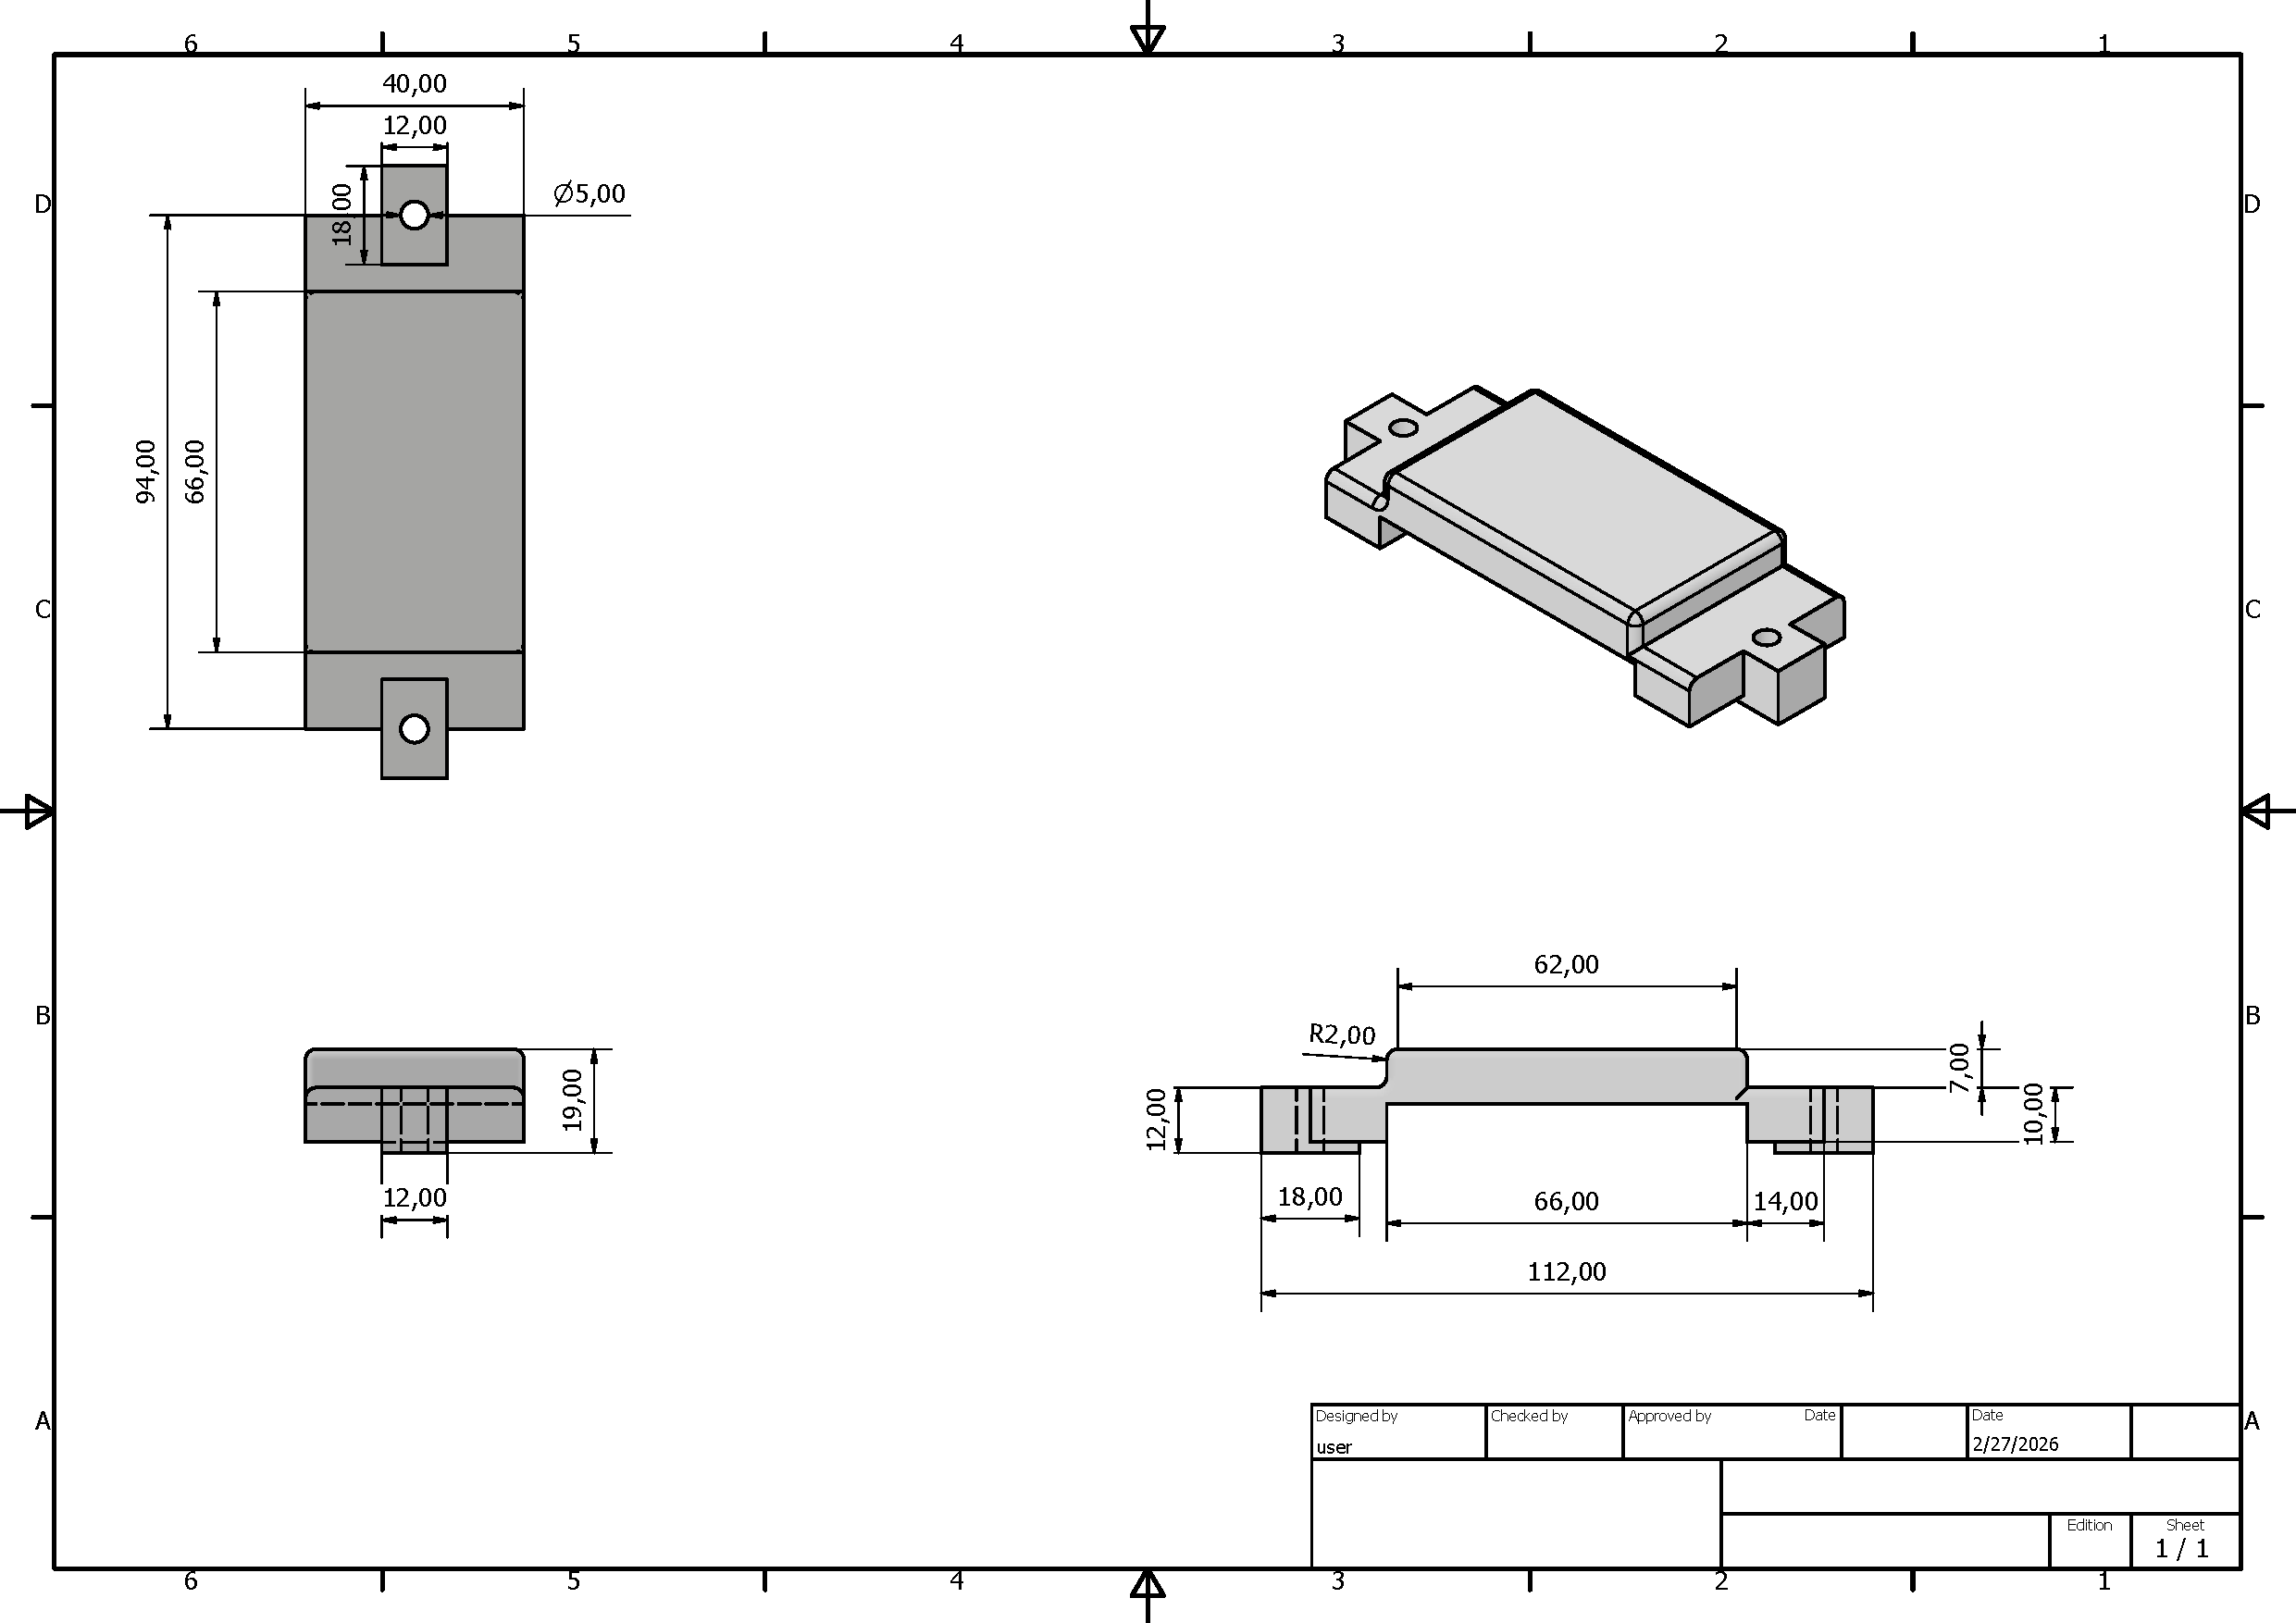
\includegraphics[width=\textwidth,page=1]{images/mechanical/18650_case_cover.pdf}
\caption{18650 battery case cover -- 2D manufacturing drawing with title block}
\label{fig:app_cad_case_cover}
\end{figure}

\begin{figure}[H]
\centering

\includegraphics[width=\textwidth,page=1]{images/mechanical/18650_case.pdf}
\caption{18650 battery case body -- 2D manufacturing drawing with title block}
\label{fig:app_cad_case_body}
\end{figure}

\begin{figure}[H]
\centering
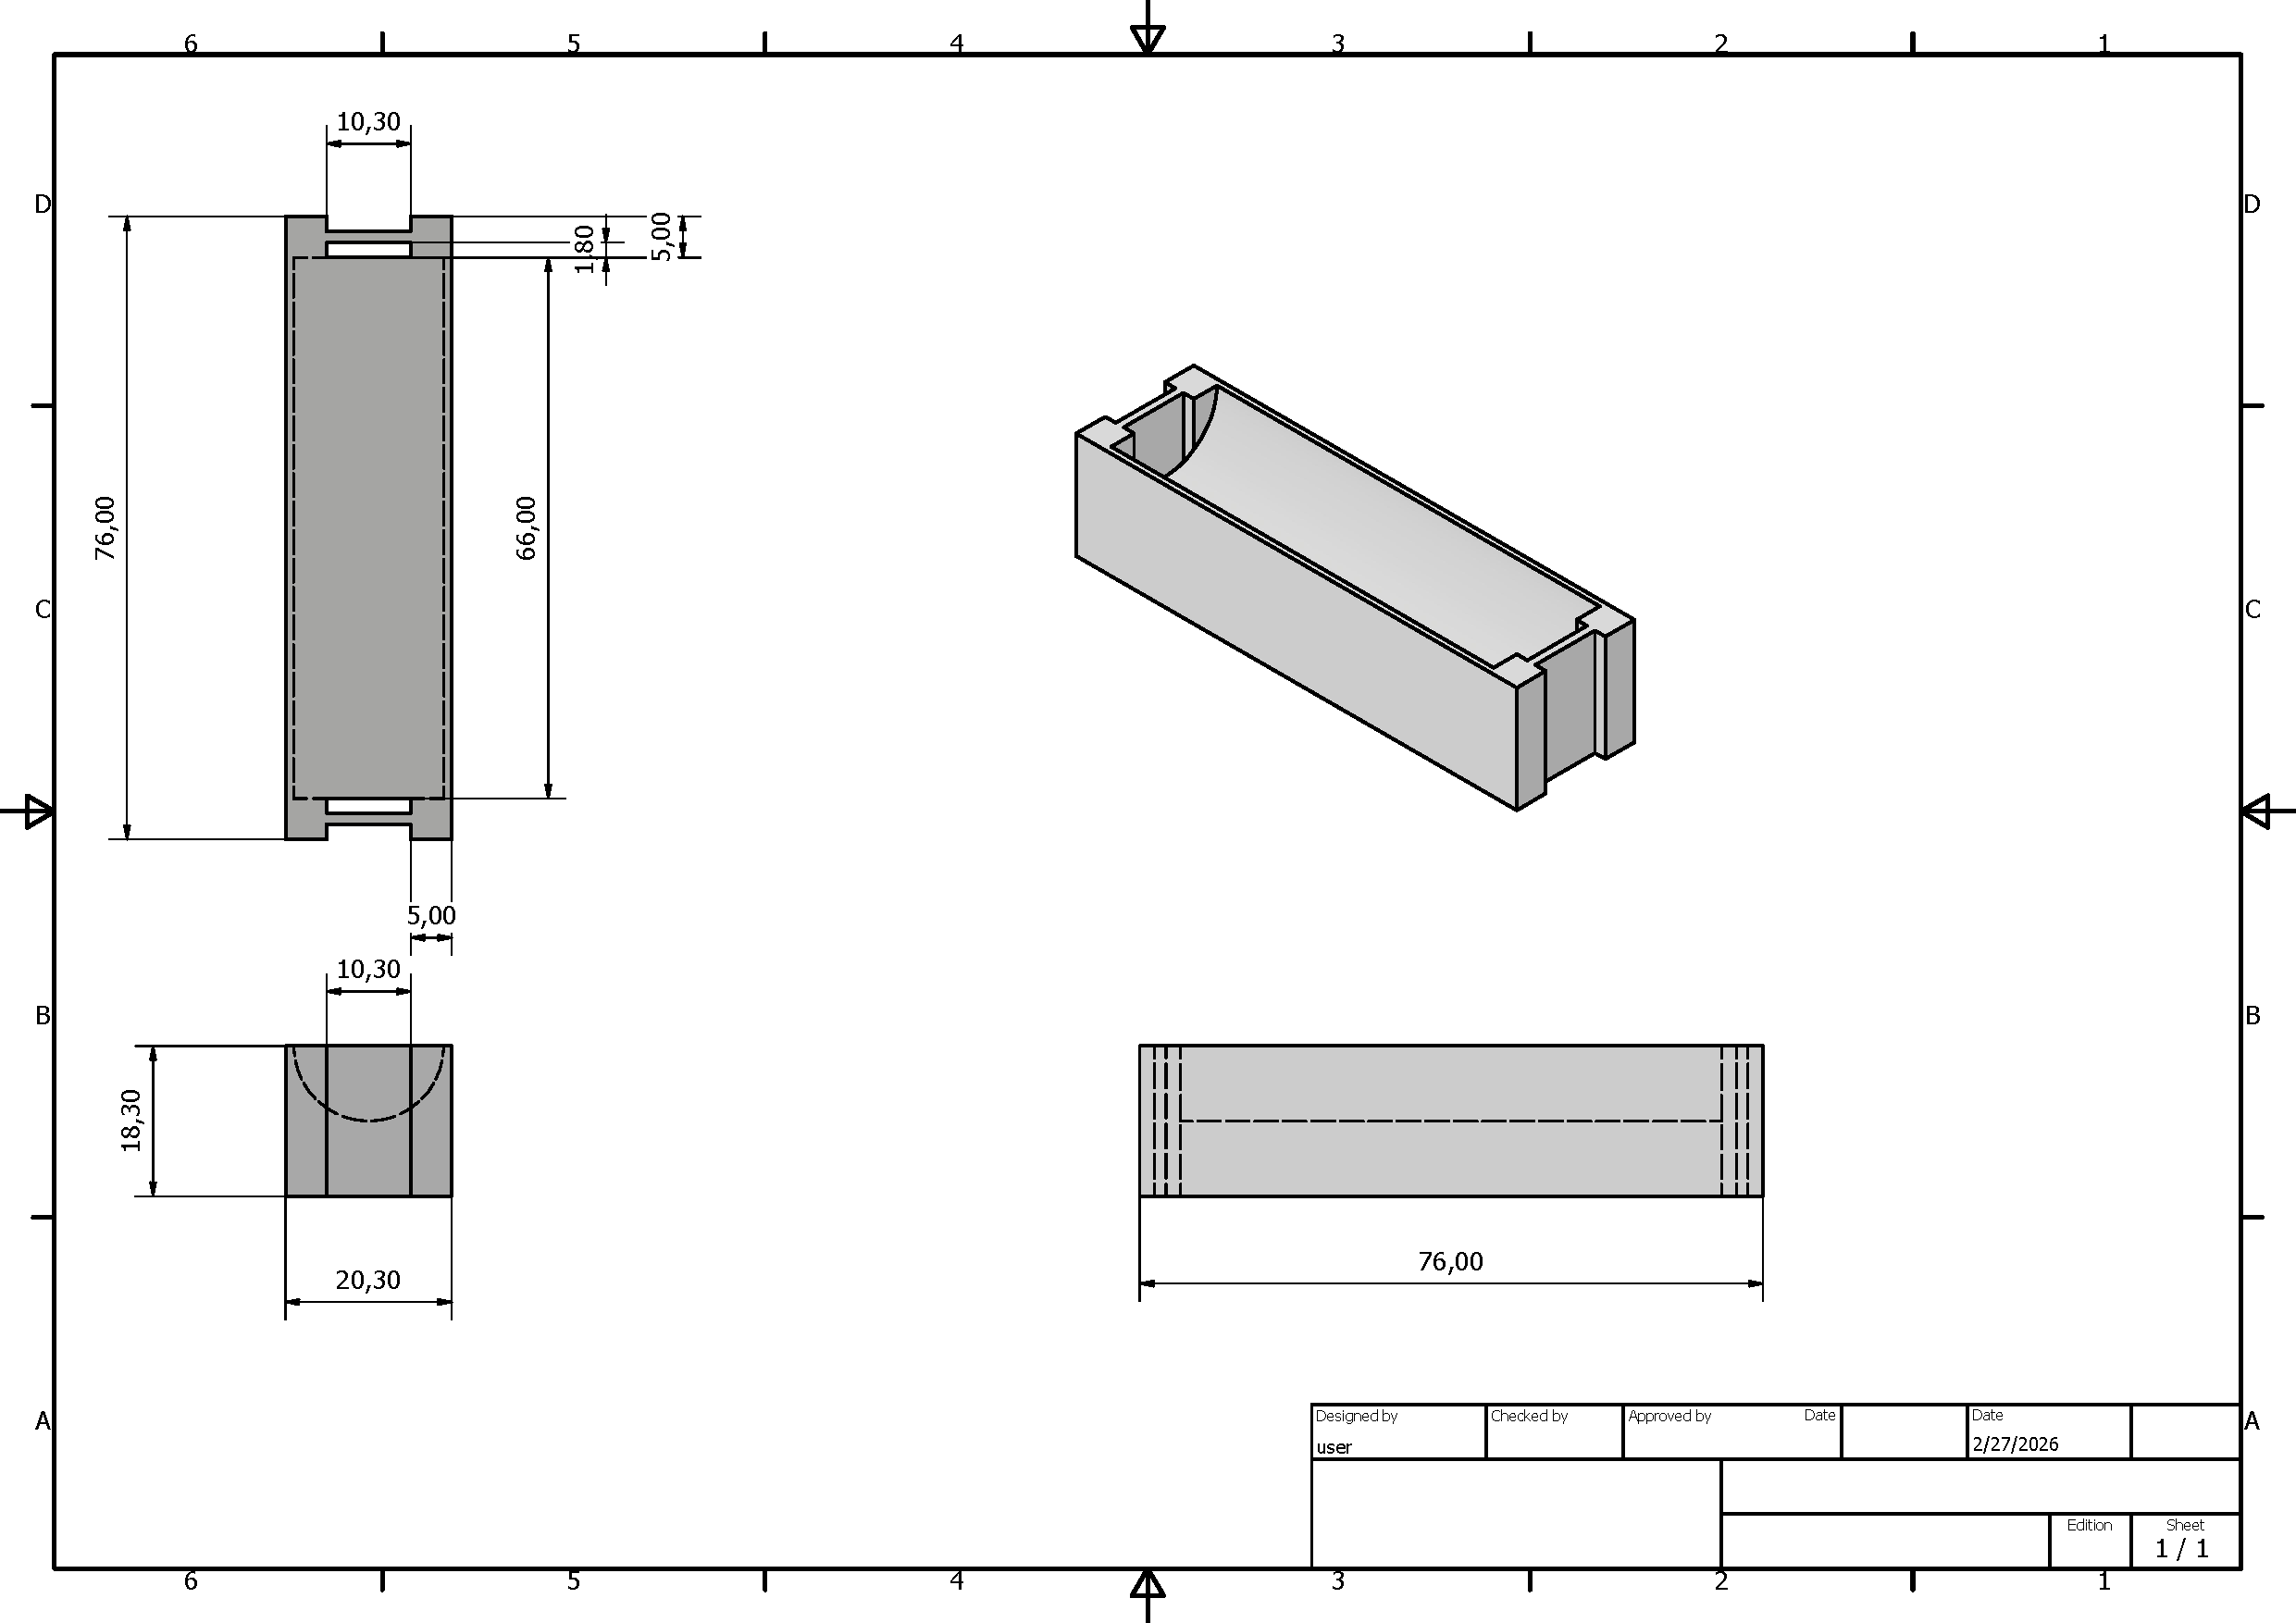
\includegraphics[width=\textwidth,page=1]{images/mechanical/Edge_Batt.pdf}
\caption{Edge battery support bracket -- 2D manufacturing drawing with title block}
\label{fig:app_cad_edge_batt}
\end{figure}

\begin{figure}[H]
\centering
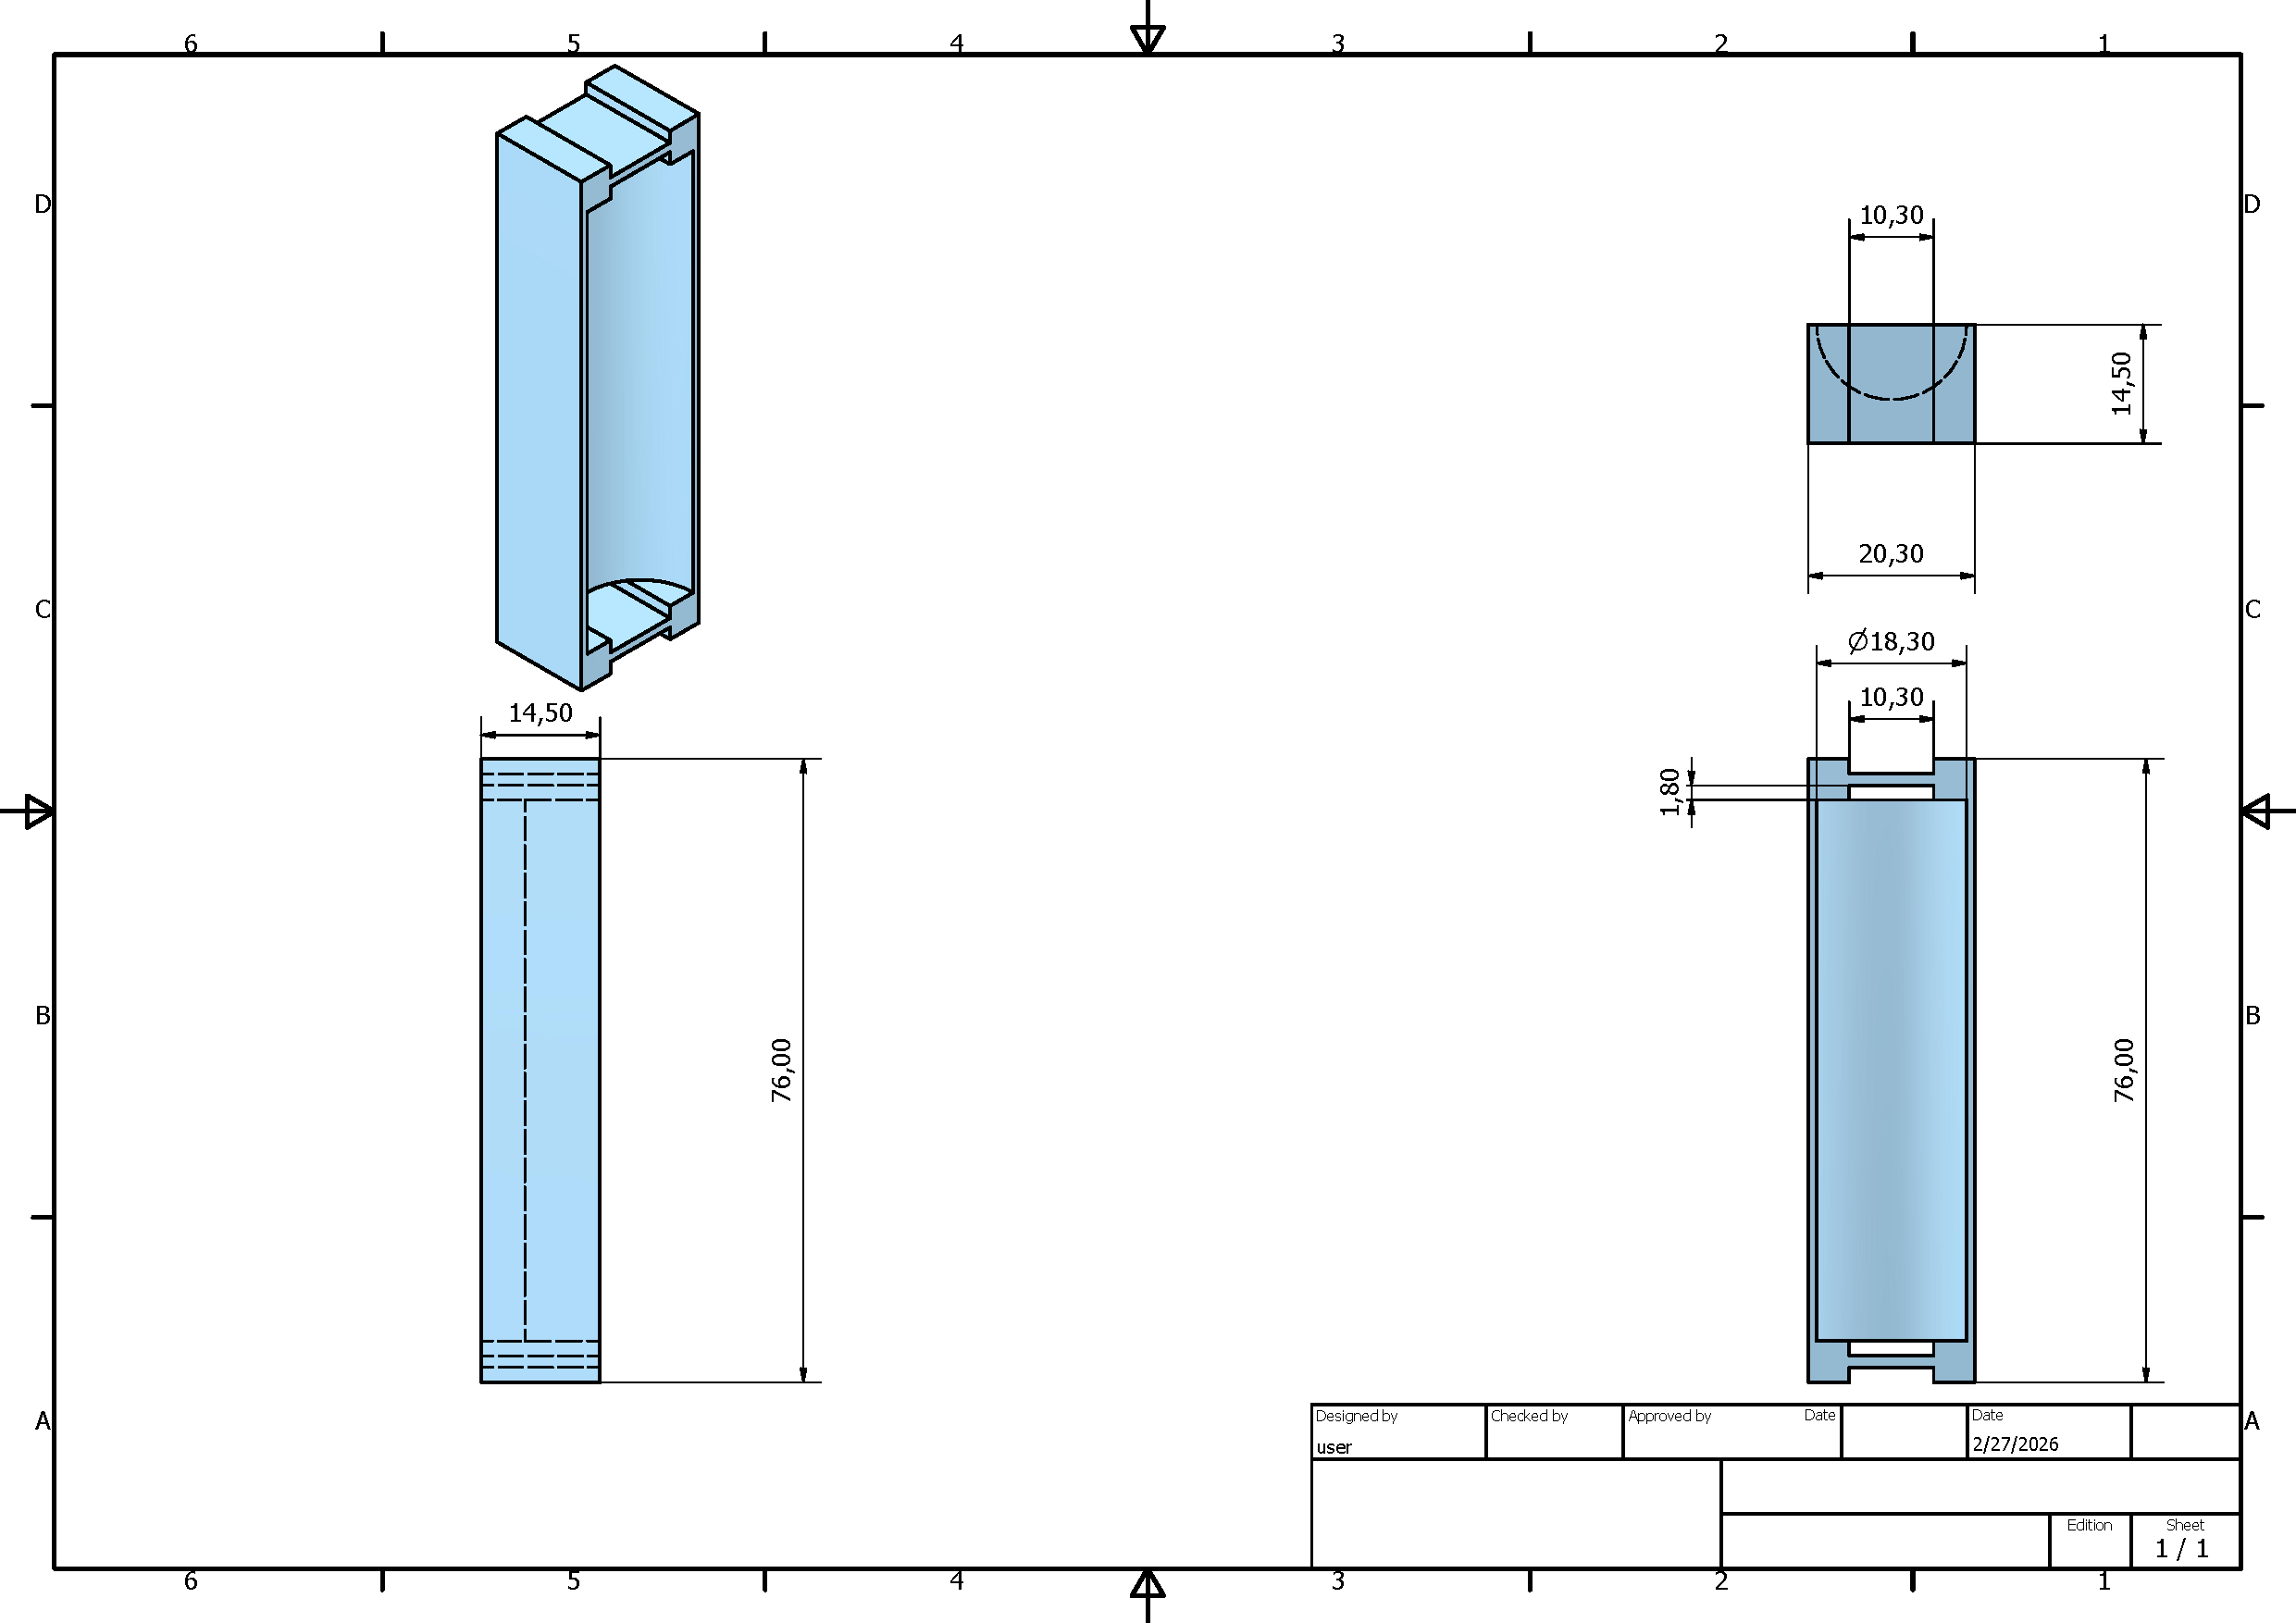
\includegraphics[width=\textwidth,page=1]{images/mechanical/mid_Batt.pdf}
\caption{Mid battery support bracket -- 2D manufacturing drawing with title block}
\label{fig:app_cad_mid_batt}
\end{figure}

% ------------------------------------------------------------
\section{Appendix B: Flight Computer Circuit Design Reference}
\label{app:fc_schematic}

Figure~\ref{fig:app_fc_easyeda} shows the current EasyEDA schematic for the flight computer, used as the design reference for PCB layout and component placement.

\begin{figure}[H]
\centering
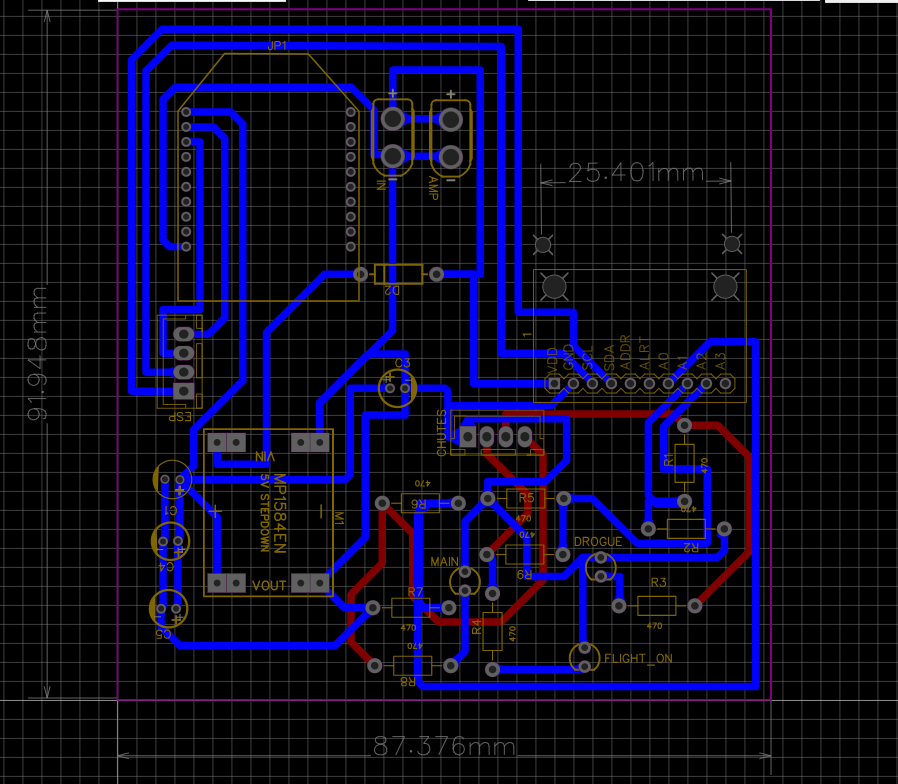
\includegraphics[width=\textwidth]{images/FC_Xbee_Design__easyDA.PNG}
\caption{Current flight computer EasyEDA schematic -- design reference for PCB fabrication (ESP32, XBee-PRO 900HP, power management, deployment circuitry)}
\label{fig:app_fc_easyeda}
\end{figure}

% ------------------------------------------------------------
\section{Appendix C: Project Budget}
\label{app:budget}

\begin{table}[H]
\centering
\caption{Project Budget Breakdown}
\small
\begin{tabular}{@{}p{4.5cm}|c|c|p{2cm}|c@{}}
\toprule
\rowcolor{gray!22}\textbf{Item} & \textbf{Qty} & \textbf{Unit Cost (KES)} & \textbf{Total (KES)} & \textbf{Status} \\ \midrule
ESP32-WROOM-32              & 2  & 1800   & 3600  & Received    \\
XBee-PRO 900HP              & 2  & 4,500 & 9,000  & Received    \\
4S Lithium ion batteries (30000 mAh) & 4  & 500 & 2000  & Received    \\
BMS Board (4S)              & 3  & 650   & 1,950  & Received    \\
IRLZ44N MOSFET              & 10 & 45    & 450    & Received    \\
Nichrome Wire (10 m)        & 1  & 500   & 500    & Received    \\
PCB Fabrication (5 pcs)     & 1  & 4,500 & 4,500  & Fabrication \\
PCB Components (R, C, etc.) & 1  & 2,000 & 2,000  & Partial     \\
PETG Filament (1 kg)        & 1  & 1,800 & 1,800  & Received    \\
Crimson Powder (100 g)        & 1  & 500   & 500    & Pending     \\
Connectors (XT60, JST, etc.)& 1  & 1,200 & 1,200  & Received    \\
Fasteners and Hardware      & 1  & 800   & 800    & Partial     \\
Miscellaneous               & 1  & 1,500 & 1,500  & --          \\ \midrule
\multicolumn{2}{r|}{\textbf{Total Estimated Cost:}} & & \textbf{37,300} & -- \\ \bottomrule
\end{tabular}
\end{table}

% ------------------------------------------------------------
\section{Appendix D: Project Timeplan}
\label{app:timeplan}

\begin{figure}[H]
\centering
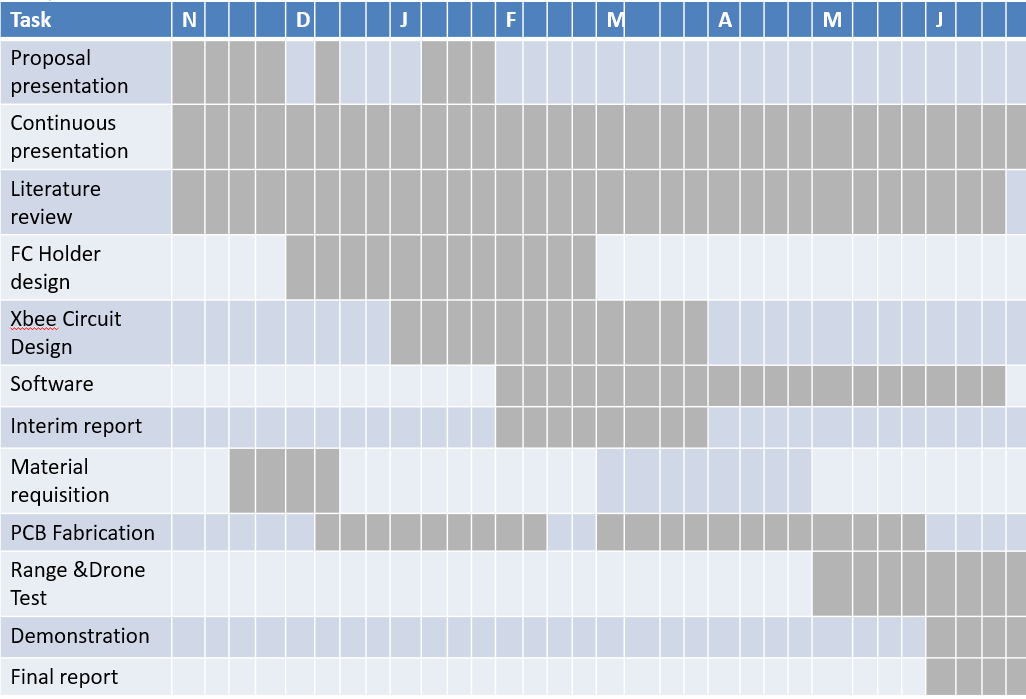
\includegraphics[width=\textwidth]{images/Timeplan.PNG}
\caption{N4 recovery system project Gantt chart showing planned phases, milestones, and current progress}
\label{fig:app_timeplan}
\end{figure}

% ============================================================
%  END OF APPENDICES
% ============================================================

\end{document}
